\documentclass[twoside,11pt]{article}

\usepackage[preprint,abbrvbib]{jmlr2e}
\usepackage[T1]{fontenc}
\usepackage{lmodern}
\usepackage{amsmath}
\usepackage{booktabs}
\usepackage{multirow}
\usepackage{graphicx}
\usepackage{xcolor}
\usepackage{lastpage}
\usepackage{float}
\usepackage{placeins}

% generated by code/make_tables.py; do not edit
\newcommand{\nItems}{5{,}421}
\newcommand{\nModels}{37}
\newcommand{\nLabelErrA}{100}
\newcommand{\errRateA}{1.84}
\newcommand{\hiddenMinA}{8}
\newcommand{\hiddenMaxA}{30}
\newcommand{\hiddenMedA}{17}
\newcommand{\inflMinA}{0.15}
\newcommand{\inflMaxA}{0.55}
\newcommand{\rankGainA}{3}
\newcommand{\favFlaggersA}{7}
\newcommand{\indepRatioA}{1.8}
\newcommand{\allPanelAdjA}{5{,}051}
\newcommand{\topTenHiddenA}{7}
\newcommand{\topTenAdjA}{2{,}164}
\newcommand{\allPanelAdjPctA}{93}
\newcommand{\hiddenTopFiveMinA}{16}
\newcommand{\hiddenTopFiveMaxA}{20}
\newcommand{\adjTopFiveMinA}{802}
\newcommand{\adjTopFiveMaxA}{1045}
\newcommand{\errRateBmin}{21.0}
\newcommand{\errRateBmax}{29.6}
\newcommand{\inflMinB}{4.9}
\newcommand{\inflMaxB}{13.9}
\newcommand{\favFlaggersBmin}{32}
\newcommand{\favFlaggersBmax}{33}
\newcommand{\rankGainBmin}{13}
\newcommand{\rankGainBmax}{27}
\newcommand{\indepRatioBmin}{4.3}
\newcommand{\indepRatioBmax}{4.9}
\newcommand{\llamaInflB}{9.7}
\newcommand{\llamaTrueRankB}{6}
\newcommand{\llamaDrRankB}{1}
\newcommand{\llamaFavB}{5}
\newcommand{\errRateBmain}{26.5}
\newcommand{\drFlagRmseA}{0.35}
\newcommand{\tpWaldCovOneA}{0.14}
\newcommand{\tpWaldCovTwentyA}{0.90}
\newcommand{\tpCpCovMinA}{0.997}
\newcommand{\tpMaxBiasA}{0.04}
\newcommand{\tpFlagRmseTenA}{0.25}
\newcommand{\tpAdjTenA}{1279}
\newcommand{\tpAdjDRA}{819}
\newcommand{\drFlagRmseB}{9.72}
\newcommand{\tpWaldCovOneB}{0.93}
\newcommand{\tpWaldCovTwentyB}{0.95}
\newcommand{\tpCpCovMinB}{0.988}
\newcommand{\tpMaxBiasB}{0.25}
\newcommand{\tpFlagRmseTenB}{1.29}
\newcommand{\tpAdjTenB}{1595}
\newcommand{\tpAdjDRB}{1170}
\newcommand{\reps}{2{,}000}
\newcommand{\hiddenGptA}{19}
\newcommand{\allocUnifOneA}{0.38}
\newcommand{\allocNeyOneA}{0.27}
\newcommand{\allocNeyPiDOneA}{0.46}
\newcommand{\eDA}{0.076}
\newcommand{\eCA}{0.0032}
\newcommand{\nDA}{819}
\newcommand{\nCA}{4602}
\newcommand{\allocUnifOneB}{1.16}
\newcommand{\allocNeyOneB}{1.03}
\newcommand{\allocNeyPiDOneB}{0.40}
\newcommand{\eDB}{0.575}
\newcommand{\eCB}{0.0976}
\newcommand{\nDB}{1170}
\newcommand{\nCB}{4251}
\newcommand{\lockGptOneB}{3.4}
\newcommand{\lockOpusOneB}{3.4}
\newcommand{\lockHiddenOneB}{676}
\newcommand{\lockHiddenLastB}{142}
\newcommand{\lockAdjOneB}{1333}
\newcommand{\lockAdjLastB}{2644}
\newcommand{\lockPanelLastB}{5}
\newcommand{\lockGptCorrectOneB}{391}
\newcommand{\lockGptRepeatOneB}{208}
\newcommand{\lockGptCorrectPpOneB}{7.2}
\newcommand{\lockGptRepeatPpOneB}{3.8}
\newcommand{\lockOpusCorrectOneB}{388}
\newcommand{\lockOpusRepeatOneB}{205}
\newcommand{\lockHiddenLastA}{4}
\newcommand{\lockAdjLastA}{2817}
\newcommand{\sensTrueRateA}{0.0041}
\newcommand{\sensPairTrueA}{0.35}
\newcommand{\sensPairDRA}{0.20}
\newcommand{\sensPairDRAabs}{0.20}
\newcommand{\sensEpsCoverA}{0.001}
\newcommand{\sensEpsSignA}{0}
\newcommand{\sensTrueRateB}{0.1240}
\newcommand{\sensPairTrueB}{0.57}
\newcommand{\sensPairDRB}{-8.65}
\newcommand{\sensPairDRBabs}{8.65}
\newcommand{\sensEpsCoverB}{0.075}
\newcommand{\sensEpsSignB}{0.075}
\newcommand{\rateEps}{0.124}
\newcommand{\rateGamma}{0.784}
\newcommand{\rateRatioMin}{0.98}
\newcommand{\rateRatioMax}{1.03}
\newcommand{\nOk}{5{,}321}
\newcommand{\nWrongGt}{100}
\newcommand{\nBadQ}{131}
\newcommand{\nMulti}{38}
\newcommand{\nNoCorrect}{36}
\newcommand{\nExpert}{32}
\newcommand{\nBadOpt}{25}
\newcommand{\nNoMatch}{10}
\newcommand{\nUnparsed}{5}
\newcommand{\nSameAsLabel}{1}
\newcommand{\nLabelDiffers}{1}
\newcommand{\helmDisagreeTotal}{29}
\newcommand{\helmDisagreeMax}{3}
\newcommand{\helmInstances}{14{,}042}
\newcommand{\invalidMax}{994}
\newcommand{\invalidMaxModel}{Mistral Large}
\newcommand{\invalidZero}{22}
\newcommand{\simCovMinA}{0.962}
\newcommand{\simWidthOneA}{11.7}
\newcommand{\simWidthFiveA}{3.2}
\newcommand{\simWidthHalfA}{0.7}
\newcommand{\simPairWidthFiveA}{6.1}
\newcommand{\simPairWidthHalfA}{1.3}
\newcommand{\simCertFiveA}{11}
\newcommand{\simCertHalfA}{50}
\newcommand{\simNoErrOneA}{84}
\newcommand{\simTrueCertA}{97}
\newcommand{\simNadjA}{36}
\newcommand{\cpWidthOneA}{16.2}
\newcommand{\waldPairCovOneA}{0.03--0.06}
\newcommand{\simCovMinB}{0.953}
\newcommand{\simWidthOneB}{29.5}
\newcommand{\simWidthFiveB}{22.0}
\newcommand{\simWidthHalfB}{10.2}
\newcommand{\simPairWidthFiveB}{26.0}
\newcommand{\simPairWidthHalfB}{13.3}
\newcommand{\simCertFiveB}{0}
\newcommand{\simCertHalfB}{3}
\newcommand{\simNoErrOneB}{0}
\newcommand{\simTrueCertB}{97}
\newcommand{\simNadjB}{35}
\newcommand{\cpWidthOneB}{26.5}
\newcommand{\waldPairCovOneB}{0.82--0.89}
\newcommand{\simWrongMax}{0}
\newcommand{\cnItems}{46{,}328}
\newcommand{\cnExcluded}{107}
\newcommand{\cnAdj}{1{,}393}
\newcommand{\cnAdjPct}{3.0}
\newcommand{\cnFlagged}{1{,}230}
\newcommand{\cnIncidental}{163}
\newcommand{\cnRefErr}{287}
\newcommand{\cnRefErrIn}{179}
\newcommand{\cnHidden}{108}
\newcommand{\cnHiddenPct}{38}
\newcommand{\cnReissChanges}{475}
\newcommand{\cnAgreeChanges}{149}
\newcommand{\cnDisagreeIn}{347}
\newcommand{\cnTau}{0.988}
\newcommand{\cnNinv}{1}
\newcommand{\cnNmodels}{21}
\newcommand{\cnHiddenAbsMax}{0.14}
\newcommand{\cnHiddenMin}{-0.02}
\newcommand{\cnHiddenMax}{+0.14}
\newcommand{\cnAdjMin}{-0.41}
\newcommand{\cnAdjMax}{-0.28}
\newcommand{\cnAllHiddenPos}{not every}
\newcommand{\cnConcRate}{0.24}
\newcommand{\cnHiddenEntrantMean}{+0.064}
\newcommand{\cnHiddenHfMean}{+0.030}
\newcommand{\cnNhf}{5}
\newcommand{\cnNentrant}{16}
\newcommand{\cnInvA}{Carreras (b) (2003)}
\newcommand{\cnInvB}{McCallum (2003)}
\newcommand{\cnInvGap}{0.03}
\newcommand{\cnPairA}{Florian (2003)}
\newcommand{\cnPairB}{Chieu (2003)}
\newcommand{\cnPairDR}{0.011}
\newcommand{\cnPairTrue}{0.188}
\newcommand{\cnPairEpsAmbig}{0.0005}
\newcommand{\cnWidthTwo}{0.39}
\newcommand{\cnEnt}{8{,}169}
\newcommand{\cnEntHiddenMin}{-0.10}
\newcommand{\cnEntHiddenMax}{+0.78}
\newcommand{\cnEntAdjMin}{-2.47}
\newcommand{\cnEntAdjMax}{-1.70}
\newcommand{\cnEntTau}{0.990}
\newcommand{\cnEntNinv}{1}
\newcommand{\cnEntInvA}{Hendrickx (2003)}
\newcommand{\cnEntInvB}{Wu (2003)}
\newcommand{\cnEntInvGap}{0.06}
\newcommand{\cnTies}{1}
\newcommand{\cnPairs}{210}
\newcommand{\cnDisagreeChanges}{326}
\newcommand{\sweepN}{37}
\newcommand{\sweepErrMin}{13.9}
\newcommand{\sweepErrMax}{70.6}
\newcommand{\sweepBestLabeler}{Claude 3 Opus}
\newcommand{\sweepBestErr}{13.9}
\newcommand{\sweepBestMedInfl}{6.1}
\newcommand{\sweepBestMaxGain}{8}
\newcommand{\sweepMedInflMin}{6.1}
\newcommand{\sweepMedInflMax}{10.9}
\newcommand{\sweepMaxGainMax}{32}
\newcommand{\sweepFavMin}{31}
\newcommand{\dupAgree}{99.85}
\newcommand{\dupDiffer}{8}


\newcommand{\Pn}{\mathbb{P}_n}
\newcommand{\E}{\mathbb{E}}
\newcommand{\1}{\mathbf{1}}
\newcommand{\DR}{\mathrm{DR}}
\newcommand{\Dset}{\Delta}
\newcommand{\Cset}{C}
\newcommand{\inv}{\perp}

% ---- author details: fill in before submission ----
\newcommand{\AuthorFull}{AUTHOR NAME}
\newcommand{\AuthorShort}{AUTHOR SURNAME}
\newcommand{\AuthorEmail}{author@example.org}
\newcommand{\AuthorAddr}{Independent Researcher}
\newcommand{\codeurl}{\url{https://github.com/unluckyjet/discrepant-resolution}}
% ----------------------------------------------------
\ShortHeadings{Discrepant Resolution in Benchmark Relabelling}{\AuthorShort}
\firstpageno{1}

\begin{document}

\title{Only Checking Where the Model Disagrees:\\ Discrepant-Resolution Bias in Benchmark Relabelling}

\author{\name \AuthorFull \email \AuthorEmail \\
       \addr \AuthorAddr}

\editor{TBD}

\maketitle

\begin{abstract}%
Benchmark audits increasingly let models choose which labels experts re-examine: only items where a model disagrees with the label are adjudicated, and all other labels are kept. Medical statistics knows this design, discrepant analysis, to be biased; we work out its consequences for model evaluation. The accuracy such an audit reports differs from the true accuracy by an exact term in the label errors the flagger shares with the benchmark. The flagger is inflated by exactly the rate of these hidden errors, no model's advantage over the flagger is ever overstated, and models that fix the flagger's shared errors are penalised. Without adjudicating some agreeing items, accuracy is not identified; we give sharp sensitivity bounds. A two-phase design that also samples agreeing items is unbiased for every model, attains the minimax rate for the flagger once enough agreeing items are adjudicated, and gives simultaneous exact intervals of near-optimal width. On MMLU with HELM predictions for \nModels{} models, a simulated audit leaves \hiddenTopFiveMinA--\hiddenTopFiveMaxA{} of \nLabelErrA{} label errors uncorrected; with labels from a language model the flagger gains \inflMinB--\inflMaxB{} points. In the published CoNLL-2003 audit, \cnHiddenPct\% of label errors were never examined, yet token accuracies shift by at most \cnHiddenAbsMax{} points.
\end{abstract}

\begin{keywords}
  discrepant analysis, benchmark evaluation, label noise, two-phase sampling, minimax lower bounds
\end{keywords}

%=====================================================================
\section{Introduction}
%=====================================================================

Benchmark labels are wrong more often than benchmark users assume. When a model disagrees with a label, the model is sometimes right. This observation has turned into a standard audit procedure. A model, an algorithm such as confident learning, or a panel of models flags the items on which it disagrees with the benchmark label. Human experts re-examine only the flagged items, correct the labels they judge wrong, and keep the original label on every unflagged item. The corrected benchmark is then used to re-estimate the accuracy of models, often including the flagging model itself, and sometimes to re-rank them.

This procedure is attractive because flagged items are where label errors concentrate, so a small adjudication budget finds many of them. It has a flaw that medical statistics identified decades ago under the name \emph{discrepant analysis}: an item on which the flagger and the label agree can still be wrong, and the procedure never looks at such items \citep{hadgu1996discrepancy,miller1998bias}. In diagnostic-test evaluation this flaw biases the new test's estimated sensitivity and specificity upwards. The standard remedy, the composite reference standard, also re-examines a sample of concordant results \citep{alonzo1999using}. Machine-learning benchmark audits differ from the clinical setting in two ways that make the problem worse. First, the quantity of interest is usually a \emph{ranking} of many models, not the accuracy of one test. Second, the flagger is often one of the models being ranked, or is closely related to them through shared training data and architectures.

The design is not a historical curiosity. Of 22 published studies that relabel or audit machine-learning benchmarks, we find that 13 send human reviewers only to items selected by model outputs for at least part of the work, and none uses a sample of the items on which the models agreed to correct the accuracies it reports (Section~\ref{sec:practice}).

This paper works out what a discrepant-resolution (DR) audit measures, when it misleads, and how to fix it at a small extra cost. Our contributions are as follows.

\begin{enumerate}
\item \textbf{An exact bias identity} (Section~\ref{sec:bias}). For any flagging rule and any model, the DR accuracy minus the true accuracy equals the mass of hidden errors (items that are unflagged and mislabelled) on which the model repeats the wrong label, minus the mass on which it gives the correct answer. Three consequences follow. The flagger's accuracy is inflated by exactly the hidden-error rate, the largest inflation possible. DR never overstates any model's advantage over the flagger. Models that correct the flagger's shared errors are penalised (\emph{lock-in}).
\item \textbf{Non-identification and sensitivity analysis} (Section~\ref{sec:ident}). DR data alone cannot determine any model's accuracy. Under an assumed bound $\varepsilon$ on the concordant label-error rate we derive sharp identified sets for accuracies and pairwise differences, which lets readers re-analyse published audits.
\item \textbf{Two-phase designs and their limits} (Section~\ref{sec:twophase}). We analyse a design that also adjudicates a random fraction of concordant items, together with a difference estimator that uses the original label as a proxy. The estimator is design-unbiased for every model, including models evaluated after the audit. We give its exact variance, an unbiased variance estimator and the Neyman allocation; intervals for the rare-error regime follow in contribution~4. For the flagger's accuracy we prove a minimax lower bound of order $\gamma\min\{\varepsilon,\sqrt{\varepsilon/m}\}$, where $\gamma$ is the fraction of concordant items, $\varepsilon$ the concordant label-error rate and $m$ the number of concordant items adjudicated. The two-phase estimator attains this rate when $m\ge1/\varepsilon$; below that, no design does better than the order $\gamma\varepsilon$ error of DR itself.
\item \textbf{Simultaneous exact intervals and a decision rule} (Sections~\ref{sec:simultaneous}--\ref{sec:rule}). A single exact hypergeometric bound on the hidden-error count, propagated through the identified set, gives finite-sample intervals for all accuracies and all pairwise differences at once, and hence certified ranking orders. In the rare-error regime their width is of order $\gamma\log(1/\alpha)/m$, and a matching lemma shows that, for the flagger and even when there are no hidden errors, no valid interval can be narrower up to constants. A per-model comparison with DR yields a pilot-free procedure: sample $m$ concordant items, and if no error appears, report DR with the sensitivity bounds at $\varepsilon\approx3/m$.
\item \textbf{Evidence on real models and labels} (Section~\ref{sec:empirical}). MMLU-Redux re-annotated a random sample of MMLU independently of any model \citep{gema2025are}. Combined with HELM's per-item predictions for \nModels{} language models \citep{liang2023holistic}, it lets us simulate the audit that a DR study would have run and compare it with the truth. We also re-analyse a published DR audit, that of CoNLL-2003 by \citet{reiss2020identifying}, against the independent full re-check CoNLL++ \citep{wang2019crossweigh}.
\end{enumerate}

Section~\ref{sec:practice} reviews how published relabelling studies adjudicate. Section~\ref{sec:related} discusses related work and Section~\ref{sec:discussion} gives practical recommendations. Proofs are in Appendix~\ref{app:proofs}. Code, derived data and the literature coding are available at \codeurl.

\begin{figure}[t]
\centering
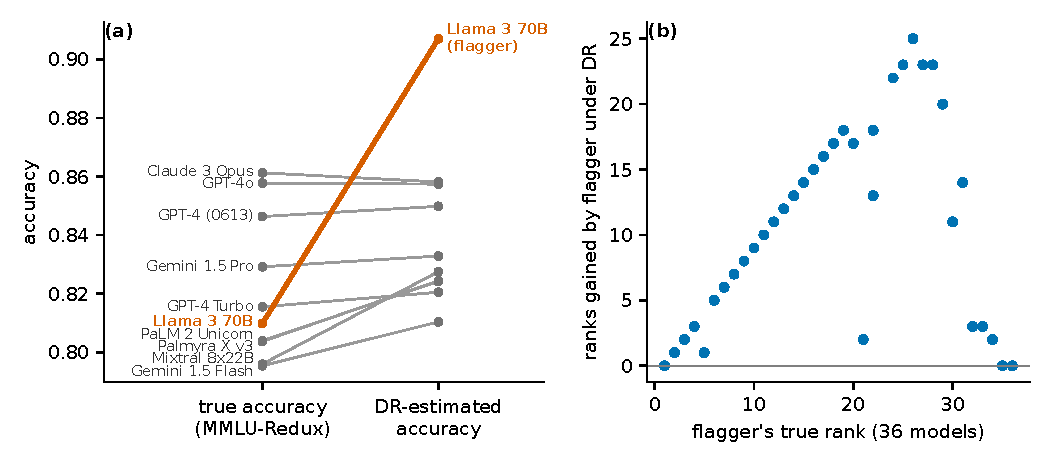
\includegraphics[width=\linewidth]{figures/fig_slope.pdf}
\caption{Discrepant resolution favours the flagger. The benchmark is the \nItems{} MMLU-Redux items, labelled by Mixtral 8x7B (\errRateBmain\% label errors); the reference labels come from a random human re-annotation. (a)~True accuracy against DR-estimated accuracy for the ten most accurate models when Llama~3~70B is the flagger. The flagger moves from rank \llamaTrueRankB{} to rank \llamaDrRankB. (b)~Ranks gained under DR for each of the 36 possible single-model flaggers, against the flagger's true rank. The gain is zero only for the most accurate model and for the weakest ones, which cannot pass the models above them.}
\label{fig:slope}
\end{figure}

%=====================================================================
\section{Setup}
\label{sec:setup}
%=====================================================================

\paragraph{Items, labels and models.} A benchmark has $n$ items indexed by $i\in[n]$. Each item has an original label $L_i\in[c]$ and a reference label $Y_i\in[c]$, the label that an adjudicator would assign; we write $c\ge 2$ for the number of classes. Models $k=1,\dots,K$ make predictions $M_{ik}\in[c]\cup\{\inv\}$, where $\inv$ denotes an invalid output that matches no label. For a property $A_i$ of items we write $\Pn(A)=n^{-1}\sum_{i}\1\{A_i\}$, the proportion of items with that property. Until Section~\ref{sec:lower} the items are fixed and all randomness comes from the adjudication design. The target of evaluation is the accuracy against the reference label,
\[
\theta_k=\Pn(M_k=Y),
\]
while the \emph{naive} accuracy is $\theta^L_k=\Pn(M_k=L)$. The reference label stands for whatever the adjudication process returns; Remark~\ref{rem:adjudicator} discusses imperfect adjudicators.

\paragraph{Discrepant resolution.} An audit chooses a set of flagged (\emph{discordant}) items $\Dset\subseteq[n]$, adjudicates exactly those items, and produces resolved labels
\[
D_i=\begin{cases}Y_i, & i\in\Dset,\\ L_i, & i\in\Cset=[n]\setminus\Dset.\end{cases}
\]
Items in $\Cset$ are \emph{concordant}. The DR accuracy of model $k$ is $\theta^\DR_k=\Pn(M_k=D)$. The main case is a \emph{single flagger} $f$, one of the models, with $\Dset=\{i:M_{if}\neq L_i\}$. A \emph{panel} $G$ of flaggers with the union rule uses $\Dset_G=\bigcup_{g\in G}\{i:M_{ig}\ne L_i\}$, flagging an item if any panel member disagrees with its label. Most results hold for an arbitrary $\Dset$, which covers confident learning and other flagging algorithms.

\paragraph{Hidden errors.} The central object is the set of \emph{hidden errors}, the mislabelled items that the audit never examines:
\[
J=\{i\in\Cset: L_i\neq Y_i\}.
\]
For a single flagger, $J=\{i: M_{if}=L_i\neq Y_i\}$ is the set of label errors that the flagger reproduces. If flagger and benchmark labels erred independently and a wrong answer chose among the $c-1$ wrong options uniformly, $\Pn(J)$ would be about $\Pn(L\neq Y)\,\Pn(M_f\neq Y)/(c-1)$. Section~\ref{sec:empirical} shows that real hidden-error rates are several times larger.

%=====================================================================
\section{What discrepant resolution measures}
\label{sec:bias}
%=====================================================================

\begin{proposition}[Bias identity]\label{prop:bias}
For any flagged set $\Dset$ and any model $k$,
\begin{equation}\label{eq:bias}
\theta^\DR_k-\theta_k \;=\; \Pn(J,\,M_k=L)\;-\;\Pn(J,\,M_k=Y).
\end{equation}
The naive bias is $\theta^L_k-\theta_k=\Pn(L\neq Y, M_k=L)-\Pn(L\neq Y, M_k=Y)$. DR therefore removes exactly the part of the naive bias that comes from flagged items and leaves the part from hidden errors untouched.
\end{proposition}

The identity is elementary (Appendix~\ref{app:proofs}), but it has sharp consequences. The bias depends on the audit only through $J$. On each hidden error, a model that repeats the wrong label gains a point it should not have, and a model that answers correctly loses a point it should have. Models that agree with the flagger on its errors therefore gain, and models that do better than the flagger lose.

\begin{corollary}[The flagger receives the largest inflation]\label{cor:flagger}
For a single flagger $f$, $\theta^\DR_f-\theta_f=\Pn(J)$, and every model $k$ satisfies $-\Pn(J)\le\theta^\DR_k-\theta_k\le\Pn(J)$.
\end{corollary}

\begin{corollary}[DR never overstates an advantage over the flagger]\label{cor:advantage}
For a single flagger $f$ and any model $k$,
\begin{equation}\label{eq:advantage}
\big(\theta^\DR_k-\theta^\DR_f\big)-\big(\theta_k-\theta_f\big)\;=\;-\Pn(J, M_k\neq L)-\Pn(J,M_k=Y)\;\le\;0 .
\end{equation}
Hence DR ranks the flagger strictly above a truly more accurate model $k$ if and only if
\[
0<\theta_k-\theta_f<\Pn(J,M_k\neq L)+\Pn(J,M_k=Y).
\]
\end{corollary}

The right-hand side of the inversion condition counts each hidden error that model $k$ answers correctly twice: once because $k$ loses it and once because the flagger gains it. A model that is better than the flagger exactly on the flagger's own blind spots is the one most likely to be ranked below it. Corollary~\ref{cor:advantage} also gives a usable one-sided statement. When a DR audit reports that model $k$ beats the flagger by $x$ points, the true advantage is at least $x$. When it reports that the flagger beats $k$, that conclusion may be an artefact of the design.

\begin{proposition}[Panels and lock-in]\label{prop:panel}
Let $G$ be a panel with the union rule and $J_G=\{i: M_{ig}=L_i\ \forall g\in G,\ L_i\neq Y_i\}$.
\begin{enumerate}
\item[(a)] If $G\subseteq G'$, then $J_{G'}\subseteq J_G$ and $\Dset_G\subseteq\Dset_{G'}$: larger panels leave fewer hidden errors but adjudicate more items.
\item[(b)] Every panel member $g\in G$ has DR bias exactly $\Pn(J_G)$. Consequently DR preserves every accuracy difference between panel members; the distortion falls on comparisons between members and non-members.
\item[(c)] A model $k\notin G$ has DR bias $\Pn(J_G,M_k=L)-\Pn(J_G,M_k=Y)$. This bias is negative whenever $k$ answers correctly on more of the panel's shared errors than it repeats.
\end{enumerate}
\end{proposition}

Part (c) is the lock-in effect. A benchmark cleaned by DR with today's models keeps exactly the errors those models share. A later model that has learned the right answers is scored as wrong on them, so it is penalised relative to the models that cleaned the benchmark. Part (a) states the cost of escaping lock-in through larger panels: the adjudicated set grows towards the whole benchmark, which removes the savings that motivated DR in the first place (Section~\ref{sec:emp-bias}).

\begin{remark}[Imperfect adjudication and other flagging rules]\label{rem:adjudicator}
If adjudication returns $A_i$, possibly different from the truth, all statements hold with $Y$ replaced by $A$, and accuracy is then measured against adjudicated labels. Measured against the truth, the same computation as in Proposition~\ref{prop:bias} gives the exact decomposition
\[
\theta^\DR_k-\theta_k=\big[\Pn(J,M_k=L)-\Pn(J,M_k=Y)\big]+\big[\Pn(\Dset,M_k=A)-\Pn(\Dset,M_k=Y)\big],
\]
a hidden-error term plus an adjudicator term. When $A$ and $Y$ come from two independent relabelings, the second term measures their disagreement and need not indicate an error of $A$. Errors of the adjudicator are a separate problem that no choice of which items to adjudicate can remove. Proposition~\ref{prop:bias} uses no property of $\Dset$, so it covers majority-vote panels, confident learning, and thresholds on model confidence. Corollaries~\ref{cor:flagger} and~\ref{cor:advantage} use only the fact that the flagger agrees with $L$ on $\Cset$.
\end{remark}

%=====================================================================
\section{Identification and sensitivity analysis}
\label{sec:ident}
%=====================================================================

A DR audit observes $O=\big(L,\,(M_k)_{k\le K},\,\Dset,\,(Y_i)_{i\in\Dset}\big)$. The reference labels of concordant items are never observed, and they are exactly what the bias depends on. Without some restriction on them, no amount of DR data pins down any accuracy.

\begin{theorem}[Sharp identified set]\label{thm:ident}
Fix $\eta\ge0$ and let $\mathcal Y(\eta)$ be the set of label vectors $y\in[c]^n$ that agree with $Y$ on $\Dset$ and satisfy $\Pn(i\in\Cset: y_i\neq L_i)\le\eta$. Write $\bar\eta=\lfloor \eta n\rfloor/n$ and $\theta_k(y)=\Pn(M_k=y)$. Then
\[
\{\theta_k(y): y\in\mathcal Y(\eta)\} = \Big[\theta^\DR_k-\min\{\bar\eta,\Pn(\Cset,M_k=L)\},\;\; \theta^\DR_k+\min\{\bar\eta,\Pn(\Cset,M_k\notin\{L,\inv\})\}\Big]\cap\tfrac1n\mathbb Z,
\]
so the bounds are sharp. For a pair of models $(k,l)$ the sharp bounds on $\theta_k-\theta_l$ are obtained by the greedy rule of Appendix~\ref{app:proofs}. Without a restriction ($\eta=\Pn(\Cset)$), the identified interval for $\theta_k$ has width $\Pn(\Cset, M_k\neq\inv)$, the share of concordant items on which $k$ gives a valid answer.
\end{theorem}

The parameter $\varepsilon=\eta/\Pn(\Cset)$, an upper bound on the label-error rate among concordant items, is the natural sensitivity parameter. Theorem~\ref{thm:ident} turns any published DR result into a family of intervals indexed by $\varepsilon$. A reader can then ask how large $\varepsilon$ must be before a claimed ranking could be reversed. By Corollary~\ref{cor:advantage}, the identified set for the difference $\theta_k-\theta_f$ between a model and the flagger always has the DR value as its lower endpoint.

%=====================================================================
\section{Two-phase designs}
\label{sec:twophase}
%=====================================================================

The non-identification result points to the fix: adjudicate some concordant items. Let each item $i$ be adjudicated independently with a known probability $\pi_i>0$ that may depend on phase-one data (the labels, the model predictions, and membership in $\Dset$) but not on $Y$. Let $R_i\in\{0,1\}$ indicate adjudication. The main case is stratified Poisson sampling with $\pi_i=\pi_\Dset$ on $\Dset$ and $\pi_i=\pi_C$ on $\Cset$. Define
\[
r_{ik}=\1\{M_{ik}=Y_i\}-\1\{M_{ik}=L_i\}\in\{-1,0,1\},
\qquad
\hat\theta_k=\theta^L_k+\frac1n\sum_{i=1}^n\frac{R_i}{\pi_i}\,r_{ik}.
\]
The estimator starts from the naive accuracy and adds an inverse-probability-weighted correction computed on the adjudicated items. It is the difference estimator of survey sampling with the original label as auxiliary variable \citep{sarndal1992model}. It is also prediction-powered inference with the original label playing the role of the prediction \citep{angelopoulos2023prediction}. Note that $r_{ik}\neq0$ only on mislabelled items. With $\pi_\Dset=1$, $\hat\theta_k$ equals the DR accuracy minus an unbiased estimate of its bias~\eqref{eq:bias}.

\begin{theorem}[Unbiasedness and variance]\label{thm:unbiased}
Under the design above, for every model $k$,
\[
\E[\hat\theta_k]=\theta_k,\qquad
\mathrm{Var}(\hat\theta_k)=\frac1{n^2}\sum_{i=1}^n\frac{1-\pi_i}{\pi_i}\,r_{ik}^2,
\]
and $\hat v_k=n^{-2}\sum_i R_i(1-\pi_i)\pi_i^{-2}r_{ik}^2$ is unbiased for the variance. The same statements hold for pairwise differences, with $r_{ik}$ replaced by $r_{ik}-r_{il}$.
\end{theorem}

Two features matter in practice. First, the design probabilities do not involve the evaluated model. The same adjudicated sample therefore yields unbiased estimates for every model, including models evaluated after the audit, provided those models are not trained or selected using the released adjudications. A DR-cleaned benchmark is biased for them by Proposition~\ref{prop:panel}(c). Second, $r_{ik}^2=\1\{L_i\neq Y_i,\,M_{ik}\in\{L_i,Y_i\}\}$, so the variance is driven entirely by the label errors in each stratum. When label errors are rare, many replicates of the phase-two sample contain none of them, $\hat v_k=0$, and Wald intervals undercover badly (Section~\ref{sec:emp-twophase}). Section~\ref{sec:simultaneous} gives exact intervals for that regime. For comparison, our tables also report a per-model interval that bounds the proportions of concordant items with $r_{ik}=\pm1$ by Bonferroni-combined Clopper--Pearson intervals (details in the code); it is superseded by Theorem~\ref{thm:simultaneous}.

\begin{proposition}[Neyman allocation]\label{prop:neyman}
Consider strata $h\in\{\Dset,\Cset\}$ with sizes $N_h$ and an expected budget $\sum_h N_h\pi_h=B$. Let $A_h=\sum_{k}\sum_{i\in h}r_{ik}^2$. The design that minimises $\sum_k\mathrm{Var}(\hat\theta_k)$ is $\pi_h=\min\{1,\lambda\sqrt{A_h/N_h}\}$, with $\lambda$ chosen to meet the budget. When no cap binds, $\pi_\Cset/\pi_\Dset=\sqrt{e_\Cset/e_\Dset}$, where $e_h=A_h/(K N_h)$ is the average rate of informative label errors in stratum $h$.
\end{proposition}

The optimal design does not in general adjudicate every flagged item: that is natural for cleaning a benchmark, but not for estimating accuracies, and conflating the two goals is the root of the problem studied here. The rates $e_h$ are unknown before adjudication and can be guessed from earlier audits. Theorem~\ref{thm:unbiased} assumes inclusion probabilities fixed by the phase-one data. If the stratum error rates are estimated from adjudications in the same sample and then used to set later probabilities, the design becomes outcome-dependent. The estimator stays unbiased if each item is weighted by its inclusion probability given the information available when it was selected, as in sequential and active designs \citep{zrnic2024active}, but the variance formula of Theorem~\ref{thm:unbiased} no longer applies as stated. We therefore use the oracle rates only to show what is achievable (Section~\ref{sec:emp-alloc}). Section~\ref{sec:rule} gives a procedure that needs no estimate of the rates.

\subsection{Rate optimality}
\label{sec:lower}

How many concordant items must be adjudicated? For the flagger with $\pi_\Dset=1$ and $\pi_\Cset=m/|\Cset|$, Theorem~\ref{thm:unbiased} gives
\begin{equation}\label{eq:upper}
\Big(\E\big[(\hat\theta_f-\theta_f)^2\big]\Big)^{1/2}=\gamma_n\sqrt{\frac{\varepsilon_n(1-\pi_\Cset)}{m}},
\qquad \gamma_n=\Pn(\Cset),\ \ \varepsilon_n=\frac{|J|}{|\Cset|}.
\end{equation}
The next theorem shows that, once $m\ge1/\varepsilon$, no design or estimator can do better than this rate, even an adaptive design that chooses which concordant items to adjudicate after seeing earlier adjudications. To state it we move to a superpopulation model. Items are drawn independently from a distribution $P$ over $(X,L,M_1,\dots,M_K,Y)$, where $X$ collects any observed features. The flagger is model $f$, $\gamma=P(M_f=L)$, and $\varepsilon\ge P(L\neq Y\mid M_f=L)$ bounds the hidden-error rate.

\begin{theorem}[Minimax lower bound]\label{thm:lower}
Let $\mathcal P(\gamma,\varepsilon)$ be the set of distributions with $P(M_f=L)=\gamma$ and $P(L\ne Y\mid M_f=L)\le\varepsilon$. Consider any design that adjudicates all discordant items and selects concordant items for adjudication by any rule based on observed data, with at most $m$ concordant adjudications in expectation. Then, for $\varepsilon\le1/2$ and every $m\ge0$,
\[
\inf_{\hat\theta}\ \sup_{P\in\mathcal P(\gamma,\varepsilon)}\ \E_P\big|\hat\theta-\theta_f(P)\big|\;\ge\;\frac{\gamma}{16\,e}\min\Big\{\varepsilon,\sqrt{\frac{\varepsilon}{m}}\Big\},
\]
where the infimum is over all estimators based on the observed data, $e$ is Euler's number, and $\sqrt{\varepsilon/0}=\infty$.
\end{theorem}

Two regimes follow. When $m\ge1/\varepsilon$, the design error~\eqref{eq:upper} of the two-phase estimator matches the lower bound up to the constant $16e$, the factor $\sqrt{1-\pi_\Cset}$, and the replacement of $(\gamma,\varepsilon)$ by their empirical counterparts. For the superpopulation target $\theta_f(P)$ the estimator also incurs the $O(n^{-1/2})$ error of sampling the items, which is present even under full adjudication; Theorem~\ref{thm:lowerfp} below gives the matching statement for the finite-population target. When $m<1/\varepsilon$, the minimax risk is of order $\gamma\varepsilon$, the same order as the bias of DR itself. The two-phase estimator is then not optimal: its standard deviation $\gamma\sqrt{\varepsilon/m}$ exceeds $\gamma\varepsilon$, while the midpoint of the identified interval of Theorem~\ref{thm:ident} attains the order $\gamma\varepsilon$ if $\varepsilon$ is known. Scenario A of Section~\ref{sec:empirical} lies largely in this regime. DR itself corresponds to $m=0$, where the worst-case error of any estimator is at least $\gamma\varepsilon/2$ however many discordant items are adjudicated (Appendix~\ref{app:proofs}). The bound is stated for the flagger; for another model the rate depends on how often it repeats the hidden errors.

The superpopulation statement leaves a gap: the design error~\eqref{eq:upper} concerns the accuracy $\theta_f$ of the fixed items, whereas Theorem~\ref{thm:lower} concerns $\theta_f(P)$. The next result closes it with a design-based bound for the finite-population target, uniformly over the possible configurations of hidden errors.

\begin{theorem}[Design-based lower bound]\label{thm:lowerfp}
Fix $n$ items with their labels $L$, predictions and flag set, and let $N_\Cset=|\Cset|$. Let $\mathcal J(\varepsilon)$ be the set of hidden-error configurations $J\subseteq\Cset$ with $|J|\le\varepsilon N_\Cset$, and let $\theta_f(J)$ be the flagger's accuracy when $J$ is the hidden-error set. Consider any design that adjudicates all discordant items and at most $m$ concordant items, selected by any rule based on observed data. Then, for $\varepsilon\le1/2$ and $m\ge2/\varepsilon$,
\[
\inf_{\hat\theta}\ \max_{J\in\mathcal J(\varepsilon)}\ \E\big|\hat\theta-\theta_f(J)\big|\;\ge\;\frac{N_\Cset-m}{n}\cdot\frac{1}{16\sqrt2\,e}\sqrt{\frac{\varepsilon}{m}}\;-\;e^{-\varepsilon N_\Cset/6},
\]
where the expectation is over the design.
\end{theorem}

Since $(N_\Cset-m)/n=\gamma_n(1-\pi_\Cset)$, this matches the design error~\eqref{eq:upper} of the two-phase estimator in its dependence on $\gamma_n$, $\varepsilon$ and $m$, for the same finite-population target. The exponential term is negligible whenever the expected number of hidden errors is more than a few dozen.

\subsection{Simultaneous exact intervals}
\label{sec:simultaneous}

The Wald intervals of Theorem~\ref{thm:unbiased} need many sampled label errors. Practitioners, however, report pairwise comparisons and whole rankings. Moreover, in the regime $m<1/\varepsilon$ the minimax error is of the order $\gamma\varepsilon$ of the hidden-error mass itself (Theorem~\ref{thm:lower}). This suggests bounding that mass directly and propagating the bound through the identified set of Theorem~\ref{thm:ident}. Because every accuracy and every difference is a function of the same unknown concordant labels, a single confidence statement about those labels covers all of them at once.

Assume $\pi_\Dset=1$ and Poisson sampling of concordant items. Let $S\subseteq\Cset$ be the sampled concordant items, $m=|S|$, $h=|\{i\in S:L_i\ne Y_i\}|$ the number of label errors found among them, and $K=|J|$ the unknown number of hidden errors. Write $\mathrm{HG}(h;N,K,m)$ for the hypergeometric distribution function: the probability of at most $h$ successes in a sample of $m$ drawn without replacement from $N$ items of which $K$ are successes. Define the exact upper confidence bound
\[
U=\max\{k:\ \mathrm{HG}(h;|\Cset|,k,m)>\alpha\},
\]
the set of items with known reference label $A=\Dset\cup S$, and the residual budget $B=U-h$. Let $\mathcal Y_B$ be the set of label vectors that agree with $Y$ on $A$ and differ from $L$ on at most $B$ items of $\Cset\setminus S$.

\begin{theorem}[Simultaneous exact intervals]\label{thm:simultaneous}
With probability at least $1-\alpha$, conditionally on $m$, the true label vector lies in $\mathcal Y_B$. Consequently, the intervals
\[
I_k=\Big[\min_{y\in\mathcal Y_B}\theta_k(y),\ \max_{y\in\mathcal Y_B}\theta_k(y)\Big],\qquad
I_{kl}=\Big[\min_{y\in\mathcal Y_B}\big(\theta_k(y)-\theta_l(y)\big),\ \max_{y\in\mathcal Y_B}\big(\theta_k(y)-\theta_l(y)\big)\Big]
\]
contain $\theta_k$ and $\theta_k-\theta_l$ for all models $k$ and all pairs $(k,l)$ simultaneously with probability at least $1-\alpha$. They are computed exactly by the greedy rule of Theorem~\ref{thm:ident}, applied to the unsampled concordant items with budget $B$. In particular, every ordering $\theta_k>\theta_l$ certified by $\min I_{kl}>0$ is correct, simultaneously for all certified pairs, with probability at least $1-\alpha$.
\end{theorem}

No union bound over models or pairs is needed, because all intervals are derived from the single event $\{K\le U\}$. The intervals are exact in the sense of finite-sample, design-based coverage. They make no assumption about how hidden errors relate to model predictions, and they rely only on the randomisation of the concordant sample. Their width is controlled by the residual budget.

\begin{proposition}[Width]\label{prop:width}
For every model, $|I_k|\le2B/n$, and for every pair, $|I_{kl}|\le4B/n$. If no label error is found in the concordant sample ($h=0$), then $B=U\le|\Cset|\log(1/\alpha)/m$. The intervals are then contained in the sharp bounds of Theorem~\ref{thm:ident} at a concordant error rate of $\log(1/\alpha)/m$, which is about $3/m$ for $\alpha=0.05$.
\end{proposition}

When hidden errors are rare, the width is governed by the sampling margin $\log(1/\alpha)/m$ rather than by $\varepsilon$: if $m<1/\varepsilon$, an interval of width $\gamma\log(1/\alpha)/m$ is wider than the hidden-error mass $\gamma\varepsilon$ that it has to account for. This is not slack in the construction. The next lemma shows that every valid interval must be this wide, even when there are no hidden errors at all.

\begin{lemma}[Width of valid intervals]\label{lem:width}
Let $N=|\Cset|$, sample $m$ concordant items by simple random sampling, and let $k^\star=\max\{k:\binom{N-k}{m}/\binom{N}{m}\ge2\alpha\}$. Any interval procedure for the flagger's accuracy that has coverage at least $1-\alpha$ for every hidden-error configuration has, when $J=\emptyset$, expected width at least $(\tfrac12-\alpha)\,k^\star/n$. Moreover $k^\star\ge\lfloor (N-m+1)\,x/(1+x)\rfloor$ with $x=\log(1/(2\alpha))/m$, so the expected width is at least about $(\tfrac12-\alpha)\,\gamma_n\log(1/(2\alpha))/m$.
\end{lemma}

Proposition~\ref{prop:width} gives width at most $\gamma_n\log(1/\alpha)/m$ for the flagger when no error is sampled, which is always the case when $J=\emptyset$. The intervals of Theorem~\ref{thm:simultaneous} are therefore minimax-optimal in width among valid intervals, up to constants, in the rare-error regime. Point estimation and interval estimation differ here. An estimator can be within order $\gamma\varepsilon$ of the truth (Theorem~\ref{thm:lower}), but no procedure can certify that without an interval of width of order $\gamma/m$. When hidden errors are common, the residual budget stays of order $\gamma\varepsilon n$ unless $\pi_\Cset$ is close to one. The intervals then remain valid but are wide, and the Wald intervals of Theorem~\ref{thm:unbiased}, whose width shrinks like $\gamma\sqrt{\varepsilon/m}$, are the better tool. The two constructions are complementary and mirror the two regimes of the lower bound.

\subsection{When is a concordant sample worth it?}
\label{sec:rule}

The flagger threshold $m>1/\varepsilon$ does not apply to every model, because the DR bias differs across models. With $\pi_\Dset=1$ and $\pi_\Cset=m/|\Cset|$, write $a_k=|J\cap\{M_k=L\}|/|\Cset|$ and $c_k=|J\cap\{M_k=Y\}|/|\Cset|$ for the rates at which model $k$ repeats and corrects the hidden errors.

\begin{proposition}[Per-model comparison with DR]\label{prop:rule}
The DR bias of model $k$ is $\gamma_n(a_k-c_k)$, and the root mean squared error of the two-phase estimator is $\gamma_n\sqrt{(1-\pi_\Cset)(a_k+c_k)/m}$. The two-phase estimator has the smaller error if and only if
\[
m>(1-\pi_\Cset)\,\frac{a_k+c_k}{(a_k-c_k)^2}.
\]
For the flagger, $a_f=\varepsilon_n$ and $c_f=0$, so the threshold is $(1-\pi_\Cset)/\varepsilon_n$. For a model that corrects about as many hidden errors as it repeats, DR is nearly unbiased and the threshold diverges.
\end{proposition}

Comparing mean squared errors, however, misses the main point. Whatever its error, a DR estimate carries no valid uncertainty statement: by Theorem~\ref{thm:ident}, DR data are compatible with any hidden-error mass up to $\Pn(\Cset)$, so no interval computed from DR data alone has guaranteed coverage. We therefore recommend the following procedure, which needs no pilot study.
\begin{enumerate}
\item Adjudicate all flagged items and a random sample of $m$ concordant items.
\item Report the two-phase estimates. If no label error appears in the concordant sample, these coincide with the DR estimates.
\item Report the simultaneous intervals of Theorem~\ref{thm:simultaneous}. If no error appears, they are no wider than the bounds of Theorem~\ref{thm:ident} at $\varepsilon=\log(1/\alpha)/m\approx3/m$ (Proposition~\ref{prop:width}).
\item If many label errors are expected in the concordant sample, as with LLM-generated labels, also report the Wald intervals. The choice should be specified before the sample is drawn.
\end{enumerate}

%=====================================================================
\section{How published relabelling studies adjudicate}
\label{sec:practice}
%=====================================================================

We coded the adjudication design of 22 published studies that relabel, audit or clean machine-learning benchmarks (Table~\ref{tab:literature}), each code backed by a verbatim methods quote checked mechanically against the paper's full text; the protocol is in the Online Appendix. The categories are DR (only items flagged by a model or algorithm are adjudicated), DR-multi (the flag is the union over a panel), CRS (flagged items plus a sample of unflagged ones), RANDOM (a sample drawn independently of models), FULL (every item) and OTHER (hybrids).

Eight studies use DR or DR-multi, and five of the six hybrids contain a step in which humans see only items selected by model outputs (one of them, SWE-Bench+, reviews only items the model solved; \citealp{aleithan2024swebench}). In all, 13 of the 22 studies adjudicate only model-selected items for at least part of the work. Of the eight DR studies, seven re-report accuracies or rankings on the corrected labels, seven evaluate a flagging model afterwards, and only four acknowledge that unflagged items can be mislabelled. \citet[p.~4]{beyer2020are} state the opposite assumption outright: ``In the event that all models agree with the original ImageNet label, we can safely retain the original without re-evaluation.''

Several studies contain evidence against that assumption. A random unflagged ImageNet image per class raised the estimated error rate of \citet{northcutt2021pervasive} from 6\% to about 20\%, but the estimate was not used to correct labels or rankings. A full review of SciFact found 3 of its 11 label errors among items the automated screen had not flagged \citep{sylvestre2026gold}. \citet{vendrow2025do} call their error counts lower bounds, since ``our approach could miss any bad question for which all LLM solutions happen to agree with the benchmark solution'', and \citet{chong2022detecting} warn that ``the cleaning process may bias any such benchmarks toward the models most similar to the model used to clean the data.'' The design closest to a composite reference standard \citep{alt2020tacred} finds an 8.9\% revision rate in a control group of items most models got right, but does not propagate it to unsampled items. Two studies re-annotate random samples, including MMLU-Redux \citep{gema2025are}, our ground truth in Section~\ref{sec:empirical}.

Sections~\ref{sec:bias}--\ref{sec:twophase} make these remarks quantitative. For single-flagger designs, Corollary~\ref{cor:advantage} implies that every reported improvement of another model over the flagger is a lower bound and every reported advantage of the flagger is suspect. Other flagging rules, item removal and multi-label scoring fall outside the corollary; for them Proposition~\ref{prop:bias} still applies when relabelled items are scored against the adjudicated label.

\begin{table}[t]
\centering
\scriptsize
\begin{tabular}{llllll}
\toprule
Study & Benchmark & Design & Flagger & Re-reports & Notes unflagged \\
 & & & evaluated & acc./ranking & may be wrong \\
\midrule
\citet{reiss2020identifying} & CoNLL-2003 & DR & yes & yes & no \\
\citet{northcutt2021pervasive} & 10 test sets (ImageNet, CIFAR, \dots) & DR & yes & yes & yes \\
\citet{vasudevan2022when} & ImageNet (multi-label) & DR & yes & yes & yes \\
\citet{chong2022detecting} & IMDB, Amazon, \dots & DR & partial & partial & yes \\
\citet{nahum2025are} & TRUE, SummEval & DR & yes & yes & no \\
\citet{ansari2026how} & 4 physics benchmarks & DR & yes & yes & no \\
\citet{beyer2020are} & ImageNet (ReaL) & DR-multi & yes & yes & no \\
\citet{vendrow2025do} & 15 subsets (GSM8K, SQuAD2.0, \dots) & DR-multi & yes & yes & yes \\
\citet{alt2020tacred} & TACRED & CRS & yes & yes & yes \\
\citet{shankar2020evaluating} & ImageNet & OTHER & yes & yes & yes \\
\citet{rucker2023cleanconll} & CoNLL-2003 & OTHER & yes & yes & yes \\
\citet{wang2024mmlupro} & MMLU-Pro & OTHER & yes & no & no \\
\citet{aleithan2024swebench} & SWE-bench & OTHER & yes & yes & no \\
\citet{ye2026scalable} & MedCalc-Bench & OTHER & no & yes & yes \\
\citet{land2026auditing} & 32 subsets (RewardBench 2, \dots) & OTHER & -- & no & yes \\
\citet{chowdhury2024introducing} & SWE-bench (Verified) & RANDOM & -- & yes & no \\
\citet{gema2025are} & MMLU (Redux) & RANDOM & -- & yes & no \\
\citet{wang2019crossweigh} & CoNLL-2003 & FULL & -- & yes & -- \\
\citet{stoica2021retacred} & TACRED & FULL & -- & yes & -- \\
\citet{zhai2026hleverified} & Humanity's Last Exam & FULL & -- & yes & -- \\
\citet{brunello2026fixing} & FOLIO, MALLS & FULL & partial & yes & -- \\
\citet{sylvestre2026gold} & SciFact & FULL & yes & yes & -- \\
\bottomrule
\end{tabular}

\caption{Adjudication designs of published benchmark relabelling and audit studies, coded from verbatim methods quotes (protocol in the Online Appendix). ``Flagger evaluated'' means that a model used to select items for adjudication is also among the models evaluated on the corrected labels. ``Notes unflagged may be wrong'' means the paper states that unflagged items can also be mislabelled; it is not applicable to full re-annotation.}
\label{tab:literature}
\end{table}


%=====================================================================
\section{Empirical study}
\label{sec:empirical}
%=====================================================================

\subsection{Data and scenarios}
\label{sec:data}

\paragraph{Reference labels.} MMLU-Redux 2.0 \citep{gema2025are} drew 100 questions uniformly at random from each of the 57 MMLU subjects \citep{hendrycks2021measuring}. Annotators then re-checked each question against external sources, independently of any model's output. This gives a sample of benchmark items whose labels were verified without regard to model disagreement, which is exactly what is needed to know the truth that a DR audit would miss. We keep the \nItems{} items whose reference label is determined:
\begin{itemize}
\item items annotated as correct, for which $Y=L$;
\item items annotated as having a wrong ground truth together with a parseable corrected answer.
\end{itemize}
We exclude items with unclear questions or options, no correct answer, multiple correct answers, or an ``expert'' flag, as well as 17 items that could not be matched or parsed (Online Appendix). This leaves \nLabelErrA{} items with a wrong MMLU label (\errRateA\%).

\paragraph{Model predictions.} HELM v1.3.0 \citep{liang2023holistic} publishes per-item predictions of \nModels{} language models on all MMLU subjects (5-shot, joint multiple-choice prompting). We match HELM instances to MMLU-Redux items on question and option text. Outputs that are not a bare option letter are counted as wrong, as HELM does.

\paragraph{Scenarios.} In \emph{Scenario A} the benchmark labels are the original MMLU labels. In \emph{Scenario B} the benchmark's labels are produced by a language model. Such benchmarks exist: the MedCalc-Bench audit of \citet{ye2026scalable} recomputed the test labels with Gemini~2.5~Pro, had a physician review 50 instances sampled from the top of the disagreement ranking, and scored newer models against the recomputed labels, with physician labels substituted on the reviewed subset. We simulate this case by taking one HELM model's answers as $L$; that model is then removed from the evaluated set. We use four labelers: Mixtral 8x7B (the main case), Llama 2 70B, GPT-3.5 Turbo and Qwen1.5 72B. Their label-error rates against MMLU-Redux are \errRateBmin--\errRateBmax\%. In both scenarios the flagger is a single model, or a panel combined by the union rule. We simulate the DR audit exactly: flagged items receive their MMLU-Redux label and all other items keep $L$. Because all reference labels are known, we can also compute every model's true accuracy.

\subsection{What discrepant resolution misses, and whom it favours}
\label{sec:emp-bias}

\begin{table}[t]
\centering
\scriptsize
\begin{tabular}{lrrrrrrr}
\toprule
Labels & Label err.\ (\%) & Hidden $|J|$ & Flagger inflation, pp & Flaggers & Max ranks & Kendall $\tau$ & $P(J)$ / indep. \\
 & & (range) & median [min, max] & favoured & gained & (range) & (median) \\
\midrule
(A) original MMLU & 1.8 & 8--30 & 0.31 [0.15, 0.55] & 7/37 & 3 & 0.99--1.00 & 1.8 \\
\midrule
Mixtral 8x7B & 26.5 & 284--698 & 10.7 [5.2, 12.9] & 33/36 & 25 & 0.80--0.98 & 4.8 \\
Llama 2 70B & 28.9 & 285--753 & 10.9 [5.3, 13.9] & 33/36 & 25 & 0.78--0.97 & 4.4 \\
GPT-3.5 Turbo & 29.6 & 274--754 & 10.3 [5.1, 13.9] & 33/36 & 27 & 0.80--0.97 & 4.3 \\
Qwen1.5 72B & 21.0 & 265--556 & 9.0 [4.9, 10.3] & 32/36 & 13 & 0.88--0.98 & 4.9 \\
\bottomrule
\end{tabular}

\caption{DR audits over all single-model flaggers. ``Hidden $|J|$'' is the number of label errors the flagger reproduces, which therefore stay uncorrected. ``Flagger inflation'' is $\theta^\DR_f-\theta_f$, which equals $\Pn(J)$ (Corollary~\ref{cor:flagger}). ``Flaggers favoured'' counts the flaggers that DR ranks above at least one truly more accurate model. ``Max ranks gained'' is the largest rank improvement of a flagger. ``$P(J)$/indep.'' is the hidden-error rate divided by the rate expected if flagger and label erred independently (Section~\ref{sec:setup}).}
\label{tab:scenarios}
\end{table}

Table~\ref{tab:scenarios} summarises DR audits over every single-model flagger. Table~\ref{tab:flaggersA} details Scenario A for the six strongest flaggers and for union panels. Proposition~\ref{prop:bias} holds exactly for every model, flagger and scenario: our code checks the identity to machine precision.

\paragraph{Scenario A: the original MMLU labels.} With one of the five most accurate models as flagger, a DR audit adjudicates \adjTopFiveMinA--\adjTopFiveMaxA{} items (15--19\% of the benchmark). It finds 80--84 of the \nLabelErrA{} label errors and leaves \hiddenTopFiveMinA--\hiddenTopFiveMaxA{} hidden. Over all \nModels{} possible flaggers, between \hiddenMinA{} and \hiddenMaxA{} label errors stay hidden. The flagger's accuracy is inflated by \inflMinA--\inflMaxA{} percentage points (pp). The hidden-error rate is a median \indepRatioA{} times the rate expected under independent errors.

In this low-noise regime the distortions are small. No strong flagger overtakes a better model, and across all flaggers the largest rank gain is \rankGainA{} places (\favFlaggersA{} of \nModels{} flaggers overtake at least one better model). Panels of the most accurate models shrink the hidden set, but slowly. The top-10 panel still leaves \topTenHiddenA{} hidden errors after adjudicating \topTenAdjA{} items, and the union of all \nModels{} models leaves none but adjudicates \allPanelAdjA{} items (\allPanelAdjPctA\% of the benchmark), little less than a full re-annotation. Smaller panels chosen with hindsight can remove all hidden errors more cheaply, but choosing them requires knowing where the errors are.

\begin{table}[t]
\centering
\scriptsize
\begin{tabular}{lrrrrrrr}
\toprule
Flagger & True rank & Adjudicated & Errors caught & Hidden $|J|$ & Inflation (pp) & Inversions & Flagger-favouring \\
\midrule
Claude 3 Opus & 1 & 802 & 83 & 17 & 0.31 & 0 & 0 \\
GPT-4o & 2 & 819 & 81 & 19 & 0.35 & 0 & 0 \\
GPT-4 (0613) & 3 & 879 & 83 & 17 & 0.31 & 0 & 0 \\
Gemini 1.5 Pro & 4 & 973 & 80 & 20 & 0.37 & 0 & 0 \\
GPT-4 Turbo & 5 & 1045 & 84 & 16 & 0.30 & 0 & 0 \\
Llama 3 70B & 6 & 1075 & 81 & 19 & 0.35 & 0 & 0 \\
\midrule
top-3 panel (union) & -- & 1291 & 87 & 13 & 0.24 & 0 & 0 \\
top-5 panel (union) & -- & 1667 & 88 & 12 & 0.22 & 0 & 0 \\
top-10 panel (union) & -- & 2164 & 93 & 7 & 0.13 & 0 & 0 \\
all models (union) & -- & 5051 & 100 & 0 & 0.00 & 0 & 0 \\
\bottomrule
\end{tabular}

\caption{Scenario A (original MMLU labels, \nLabelErrA{} label errors among \nItems{} items): DR audits with the six most accurate models as single flaggers, and with union panels of the top 3, 5, 10 and all models. ``Inflation'' is the flagger's DR bias; for panels it is the largest bias among panel members, which equals $\Pn(J_G)$ (Proposition~\ref{prop:panel}). ``Inversions'' counts model pairs whose order DR reverses. Online Appendix Table~OA.1 lists all \nModels{} flaggers.}
\label{tab:flaggersA}
\end{table}

\paragraph{Scenario B: a benchmark labelled by a language model.} When the labels come from a language model, hidden errors are common and DR's bias becomes large. Flagger inflation ranges from \inflMinB{} to \inflMaxB{}~pp. Between \favFlaggersBmin{} and \favFlaggersBmax{} of the 36 flaggers are ranked above at least one truly better model, and a flagger gains up to \rankGainBmin--\rankGainBmax{} places, depending on the labeler. The hidden-error rate is \indepRatioBmin--\indepRatioBmax{} times the independence prediction, because language models share their mistakes.

Figure~\ref{fig:sweep} extends this to all \sweepN{} models as labelers. Their label-error rates range from \sweepErrMin\% (\sweepBestLabeler) to \sweepErrMax\%. Even the best labeler gives a median flagger inflation of \sweepBestMedInfl~pp and a largest rank gain of \sweepBestMaxGain. Across labelers, the median inflation ranges from \sweepMedInflMin{} to \sweepMedInflMax~pp, and at least \sweepFavMin{} of the 36 flaggers overtake a better model. The original MMLU labels sit far below all language-model labelers. The two outlying maxima of about 20~pp come from a near-duplicate pair: PaLM~2 Unicorn and Palmyra X v3 give the same answer on \dupAgree\% of items (all but \dupDiffer). When one labels and the other flags, the audit corrects almost nothing.

Figure~\ref{fig:slope}(a) shows one audit: with Mixtral 8x7B labels and Llama~3~70B as flagger, DR inflates the flagger by \llamaInflB~pp and moves it from rank \llamaTrueRankB{} to rank \llamaDrRankB. Figure~\ref{fig:slope}(b) shows that rank gains are largest for flaggers of middling accuracy. Those flaggers have many truly better models to overtake and enough hidden errors to do it.

\begin{figure}[t]
\centering
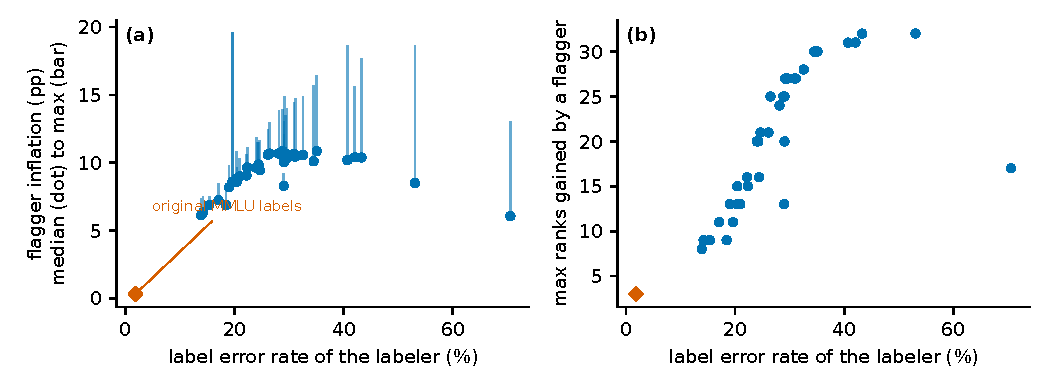
\includegraphics[width=\linewidth]{figures/fig_sweep.pdf}
\caption{Labeler-strength sweep. Each blue point is a benchmark labelled by one of the \sweepN{} HELM models (Scenario B), audited by DR with each of the other 36 models as flagger; the red diamond is Scenario A. (a)~Median flagger inflation (dot) up to the largest (bar). (b)~Largest number of ranks gained by any flagger.}
\label{fig:sweep}
\end{figure}

\subsection{Lock-in}
\label{sec:emp-lockin}

\begin{figure}[t]
\centering
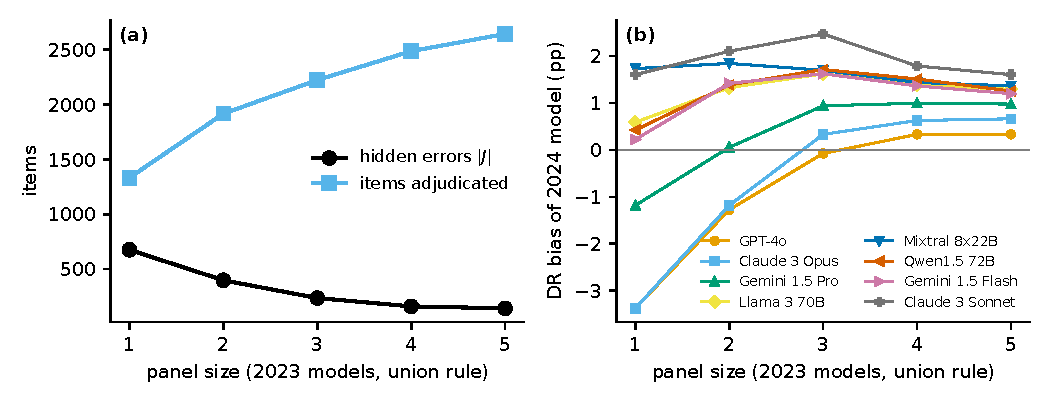
\includegraphics[width=\linewidth]{figures/fig_lockin.pdf}
\caption{Lock-in in Scenario B (Mixtral 8x7B labels). A panel of models released in 2023 cleans the benchmark by DR, and models released in 2024 are evaluated on the result. (a) Hidden errors and adjudicated items as the panel grows (panel order: GPT-3.5 Turbo, Llama 2 70B, Claude 2.1, PaLM 2 Bison, Claude Instant 1.2). (b) DR bias of the 2024 models. With a single flagger, the two strongest 2024 models, GPT-4o and Claude 3 Opus, are each underestimated by a net \lockGptOneB~pp.}
\label{fig:lockin}
\end{figure}

Proposition~\ref{prop:panel}(c) predicts that models built after an audit are penalised on the errors the auditing models share. Figure~\ref{fig:lockin} tests this by cleaning the Scenario B benchmark with models released in 2023 and evaluating models released in 2024. With GPT-3.5 Turbo as the only flagger, \lockHiddenOneB{} label errors stay hidden. GPT-4o answers \lockGptCorrectOneB{} of them correctly and is scored wrong on each, costing it \lockGptCorrectPpOneB~pp. It repeats the wrong label on \lockGptRepeatOneB{} others and is credited for them (\lockGptRepeatPpOneB~pp), so it is underestimated by a net \lockGptOneB~pp. Claude~3~Opus is underestimated by the same net amount (\lockOpusCorrectOneB{} correct answers and \lockOpusRepeatOneB{} repetitions; the two differences coincide). Weaker 2024 models that repeat more of the hidden errors are instead overestimated. Growing the panel to \lockPanelLastB{} models reduces the hidden errors to \lockHiddenLastB{}, but doubles the adjudicated set from \lockAdjOneB{} to \lockAdjLastB{} items. Some bias remains for every 2024 model, now positive, because the surviving hidden errors are the ones most models share. In Scenario A the same experiment leaves \lockHiddenLastA{} hidden errors after adjudicating \lockAdjLastA{} items, and the effect is negligible.

\subsection{A published audit: CoNLL-2003}
\label{sec:emp-conll}

\begin{table}[t]
\centering
\scriptsize
\begin{tabular}{lrrrrrrrrr}
\toprule
 & \multicolumn{2}{c}{Token accuracy (\%)} & \multicolumn{3}{c}{DR bias (pp)} & \multicolumn{2}{c}{Hidden errors} & \multicolumn{2}{c}{Rank} \\
\cmidrule(lr){2-3}\cmidrule(lr){4-6}\cmidrule(lr){7-8}\cmidrule(lr){9-10}
Model & CoNLL++ & DR & total & hidden & disagr. & correct & repeat & true & DR \\
\midrule
RoBERTa-large (J.-B.) & 98.97 & 98.57 & -0.40 & -0.017 & -0.382 & 57 & 49 & 1 & 1 \\
BERT-large (dbmdz) & 98.81 & 98.52 & -0.29 & +0.045 & -0.337 & 42 & 63 & 2 & 2 \\
BERT-large (dslim) & 98.75 & 98.42 & -0.33 & +0.017 & -0.345 & 49 & 57 & 3 & 3 \\
BERT-base (dslim) & 98.65 & 98.38 & -0.27 & +0.045 & -0.317 & 41 & 62 & 4 & 4 \\
DistilBERT (elastic) & 98.28 & 98.00 & -0.27 & +0.060 & -0.332 & 36 & 64 & 5 & 5 \\
Florian (2003) & 97.91 & 97.51 & -0.40 & +0.019 & -0.414 & 39 & 48 & 6 & 6 \\
Chieu (2003) & 97.72 & 97.50 & -0.22 & +0.108 & -0.326 & 25 & 75 & 7 & 7 \\
Klein (2003) & 97.43 & 97.25 & -0.18 & +0.138 & -0.317 & 13 & 77 & 8 & 8 \\
Zhang (2003) & 97.28 & 97.01 & -0.27 & +0.041 & -0.307 & 38 & 57 & 9 & 9 \\
Curran (2003) & 97.13 & 96.87 & -0.26 & +0.054 & -0.315 & 35 & 60 & 10 & 10 \\
Munro (2003) & 97.07 & 96.83 & -0.24 & +0.063 & -0.302 & 34 & 63 & 11 & 11 \\
Carreras (a) (2003) & 97.03 & 96.78 & -0.25 & +0.041 & -0.296 & 27 & 46 & 12 & 12 \\
Mayfield (2003) & 97.02 & 96.78 & -0.25 & +0.093 & -0.341 & 23 & 66 & 13 & 12 \\
Bender (2003) & 96.99 & 96.73 & -0.26 & +0.017 & -0.276 & 43 & 51 & 14 & 14 \\
Carreras (b) (2003) & 96.70 & 96.43 & -0.28 & +0.056 & -0.335 & 25 & 51 & 15 & 16 \\
McCallum (2003) & 96.68 & 96.43 & -0.24 & +0.101 & -0.343 & 24 & 71 & 16 & 15 \\
Hendrickx (2003) & 96.57 & 96.29 & -0.28 & +0.028 & -0.309 & 42 & 55 & 17 & 17 \\
Wu (2003) & 96.46 & 96.16 & -0.30 & +0.088 & -0.391 & 23 & 64 & 18 & 18 \\
De Meulder (2003) & 96.42 & 96.08 & -0.34 & +0.028 & -0.367 & 42 & 55 & 19 & 19 \\
Whitelaw (2003) & 96.14 & 95.84 & -0.30 & +0.050 & -0.350 & 35 & 58 & 20 & 20 \\
Hammerton (2003) & 92.13 & 91.93 & -0.20 & +0.091 & -0.294 & 29 & 71 & 21 & 21 \\
\bottomrule
\end{tabular}

\caption{Re-analysis of the published DR audit of CoNLL-2003 \citep{reiss2020identifying} against the independent full re-check CoNLL++ \citep{wang2019crossweigh}. Items are the \cnItems{} test tokens, labelled with their entity type. ``DR'' is accuracy against Reiss et al.'s resolved labels; ``CoNLL++'' is accuracy against the reference. The DR bias splits exactly into the hidden-error term and a term measuring disagreement between the two relabelings on audited tokens (Remark~\ref{rem:adjudicator}). ``Correct''/``repeat'' count the \cnHidden{} hidden errors on which a model gives the reference label or repeats the original one. Systems marked 2003 are CoNLL-2003 shared-task entries, whose outputs formed one of the audit's flagging ensembles; the others are later public transformer models. Appendix Table~\ref{tab:conllentity} repeats the analysis on entity tokens.}
\label{tab:conll}
\end{table}

The analyses so far simulate audits. We now re-analyse a published one. \citet{reiss2020identifying} audited CoNLL-2003 with three model ensembles. They reviewed the entities on which few ensemble members agreed with the label and the spans that many members proposed but the label lacked, and they corrected some nearby labels they noticed along the way. Their release includes every candidate, every verdict and the corrections. CoNLL++ \citep{wang2019crossweigh} is an independent re-check of every test sentence by two annotators, with a final round where their annotations and the original disagreed; it used no model flags. Reiss et al.\ cite it only to compare error rates, and their candidates come only from their own ensembles. Both files contain the same 46{,}435 test tokens in the same order. We exclude \cnExcluded{} tokens affected by tokenization or sentence-boundary corrections, which CoNLL++ does not make, leaving \cnItems. The original uses IOB1 tags and CoNLL++ uses BIO2.

We therefore take the token as the item and its entity type (none, person, location, organisation, miscellaneous) as the label, so the tag scheme does not matter. The adjudicated set $\Dset$ is every token covered by a span that Reiss et al.\ reviewed or corrected: \cnAdj{} tokens (\cnAdjPct\%), of which \cnIncidental{} were reviewed only incidentally. We apply their label corrections with their own code. The models are the \cnNentrant{} shared-task systems and \cnNhf{} public transformer models (Table~\ref{tab:conll}).

Against CoNLL++, \cnRefErr{} tokens of the original test set have the wrong entity type. Only \cnRefErrIn{} of them lie in the audited set; \cnHidden{} (\cnHiddenPct\%) were never examined. Because the CoNLL++ annotators corrected the existing labels rather than labelling blind, their annotations are anchored towards the original, and \cnHidden{} is probably a lower bound on the hidden errors. The two expert relabelings also disagree on many audited tokens. Reiss et al.\ changed \cnReissChanges{} token types and CoNLL++ agrees with \cnAgreeChanges{} of those changes, leaving \cnDisagreeChanges{} tokens on which the two disagree, more than all the label errors that CoNLL++ finds. We do not know which relabeling is right on those tokens; the same anchoring means that some of them may be errors that CoNLL++ missed. We therefore call the second term of the decomposition the \emph{disagreement term}, not an error of the audit.

Table~\ref{tab:conll} decomposes each model's DR bias exactly. The hidden-error term ranges from \cnHiddenMin{} to \cnHiddenMax~pp. It is positive for all models but RoBERTa-large, the strongest and most recent model, which answers more hidden errors correctly than it repeats. It averages \cnHiddenEntrantMean~pp for the 2003 systems, one of whose ensembles flagged the audit, and \cnHiddenHfMean~pp for the later models. This is consistent with lock-in, although the two ranges overlap. The 2003 systems do not share one bias, as Proposition~\ref{prop:panel}(b) would require of a union panel, because Reiss et al.\ flagged by vote thresholds rather than by the union rule. The disagreement term, from \cnAdjMin{} to \cnAdjMax~pp, dominates the total. Rankings are nearly unchanged. Kendall's $\tau_b$, which accounts for the \cnTies{} tie in the DR ranking, is \cnTau, with \cnNinv{} inversion among the \cnPairs{} pairs, between \cnInvA{} and \cnInvB, which differ by \cnInvGap~pp. This is consistent with \citet{reiss2020identifying}, who report no change in ranking.

Token accuracy is dominated by non-entity tokens, which dilutes every effect. Restricting the items to the \cnEnt{} tokens whose original or reference label is an entity, a subset fixed in advance that contains every label error, the hidden-error term ranges from \cnEntHiddenMin{} to \cnEntHiddenMax~pp and the disagreement term from \cnEntAdjMin{} to \cnEntAdjMax~pp. Kendall's $\tau_b$ is \cnEntTau, with \cnEntNinv{} inversion (\cnEntInvA{} and \cnEntInvB, \cnEntInvGap~pp apart; Appendix Table~\ref{tab:conllentity}). The effects scale with the smaller denominator, but the picture is the same.

Read with Theorem~\ref{thm:ident}, the published audit says less than its point estimates suggest. At an assumed concordant error rate of $0.2\%$, close to the true \cnConcRate\%, the identified interval for the most accurate model is \cnWidthTwo~pp wide. The audit puts \cnPairA{} \cnPairDR~pp ahead of \cnPairB, against \cnPairTrue~pp in truth, and the identified set for that difference contains zero once $\varepsilon\ge\cnPairEpsAmbig$. On this benchmark, then, hidden errors are real (more than a third of the label errors) but move token accuracies by at most \cnHiddenAbsMax~pp. The larger uncertainty comes from disagreement between expert relabelings, which no choice of items to adjudicate can remove.

\subsection{Two-phase estimation}
\label{sec:emp-twophase}

\begin{figure}[t]
\centering
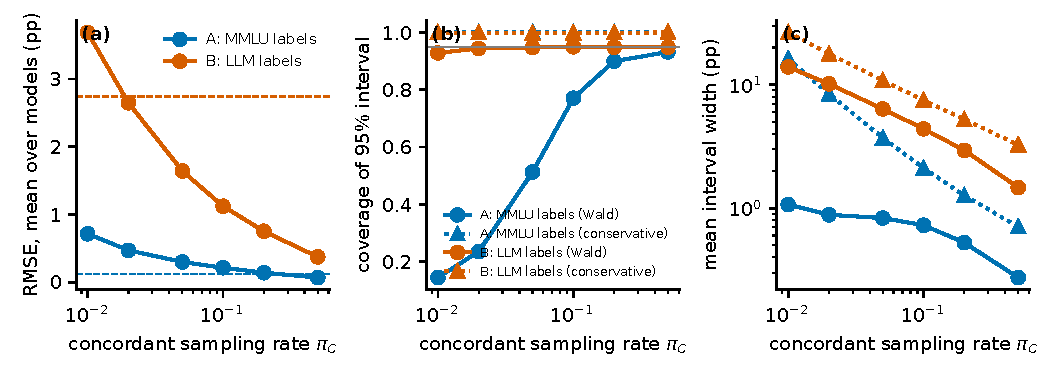
\includegraphics[width=\linewidth]{figures/fig_two_phase.pdf}
\caption{Two-phase estimation with $\pi_\Dset=1$ and concordant sampling rate $\pi_C$, over \reps{} replicates of the phase-two sample (flagger GPT-4o in Scenario A; Llama 3 70B in Scenario B with Mixtral 8x7B labels). (a)~RMSE averaged over models; dashed lines show DR ($\pi_C=0$). (b)~Coverage of nominal 95\% Wald and conservative (Clopper--Pearson) intervals, averaged over models. (c)~Mean interval widths.}
\label{fig:twophase}
\end{figure}

\begin{table}[t]
\centering
\scriptsize
\begin{tabular}{llrrrrrrrr}
\toprule
 & & & & & & \multicolumn{2}{c}{Wald} & \multicolumn{2}{c}{Conservative (CP)} \\
\cmidrule(lr){7-8}\cmidrule(lr){9-10}
Sc. & $\pi_C$ & Adjudicated & $|\text{bias}|$ & RMSE & RMSE$_F$ & cover & width & cover & width \\
\midrule
\multirow{7}{*}{A} & DR ($\pi_C=0$) & 819 & 0.125 & 0.13 & 0.35 & -- & -- & -- & -- \\
 & 0.01 & 865 & 0.014 & 0.72 & 0.80 & 0.145 & 1.07 & 1.000 & 16.22 \\
 & 0.02 & 911 & 0.016 & 0.47 & 0.53 & 0.235 & 0.88 & 1.000 & 8.42 \\
 & 0.05 & 1049 & 0.006 & 0.30 & 0.34 & 0.513 & 0.83 & 1.000 & 3.71 \\
 & 0.1 & 1279 & 0.004 & 0.22 & 0.25 & 0.771 & 0.73 & 1.000 & 2.12 \\
 & 0.2 & 1739 & 0.002 & 0.14 & 0.16 & 0.900 & 0.53 & 1.000 & 1.27 \\
 & 0.5 & 3120 & 0.001 & 0.07 & 0.08 & 0.932 & 0.27 & 1.000 & 0.71 \\
\midrule
\multirow{7}{*}{B} & DR ($\pi_C=0$) & 1170 & 2.740 & 2.74 & 9.72 & -- & -- & -- & -- \\
 & 0.01 & 1213 & 0.094 & 3.68 & 4.15 & 0.929 & 13.92 & 1.000 & 26.48 \\
 & 0.02 & 1255 & 0.040 & 2.65 & 2.95 & 0.944 & 10.15 & 0.999 & 17.81 \\
 & 0.05 & 1382 & 0.029 & 1.64 & 1.85 & 0.947 & 6.37 & 0.999 & 10.81 \\
 & 0.1 & 1595 & 0.028 & 1.12 & 1.29 & 0.950 & 4.39 & 0.999 & 7.49 \\
 & 0.2 & 2020 & 0.017 & 0.75 & 0.85 & 0.949 & 2.94 & 1.000 & 5.24 \\
 & 0.5 & 3296 & 0.007 & 0.38 & 0.42 & 0.949 & 1.47 & 1.000 & 3.26 \\
\bottomrule
\end{tabular}

\caption{Two-phase estimation over \reps{} phase-two replicates; the DR row is deterministic. ``Adjudicated'' is the mean number of adjudicated items. $|\text{bias}|$ and RMSE are averaged over models, in pp; RMSE$_F$ is the flagger's RMSE. Coverage and width refer to nominal 95\% intervals averaged over models.}
\label{tab:twophase}
\end{table}

We simulate the phase-two sample \reps{} times for each concordant sampling rate $\pi_C$, keeping the items fixed and adjudicating all discordant items. Results are in Figure~\ref{fig:twophase} and Table~\ref{tab:twophase}.

The estimator is unbiased, as Theorem~\ref{thm:unbiased} states: the largest Monte Carlo bias over models and sampling rates is \tpMaxBiasA~pp in Scenario A and \tpMaxBiasB~pp in Scenario B. Removing the bias costs some adjudication. In Scenario B, DR's error for the flagger is \drFlagRmseB~pp. With $\pi_C=0.1$ the two-phase estimator reduces it to \tpFlagRmseTenB~pp RMSE, adjudicating on average \tpAdjTenB{} items instead of \tpAdjDRB.

Scenario A shows the limits of the approach when label errors are rare. Only \hiddenGptA{} of the \nCA{} concordant items are mislabelled, so DR's bias is small: \drFlagRmseA~pp for the flagger. At small $\pi_C$ most phase-two samples contain no hidden error at all. The unbiased estimator then has a larger RMSE than DR, and its plug-in variance is often zero, so Wald intervals undercover severely (coverage \tpWaldCovOneA{} at $\pi_C=0.01$ and \tpWaldCovTwentyA{} at $\pi_C=0.2$). The conservative intervals cover in both scenarios (coverage at least \tpCpCovMinA{} in A and \tpCpCovMinB{} in B), at the price of width.

In this regime, then, the honest summary of a DR audit is not a corrected accuracy. It is a corrected accuracy together with an interval wide enough to reflect how little has been learned about concordant items, which is what the simultaneous intervals of Theorem~\ref{thm:simultaneous} provide (Section~\ref{sec:emp-sim}). This is also the regime $m<1/\varepsilon$ of Theorem~\ref{thm:lower}, in which no design can estimate accuracies to better than the order of DR's own bias.

\subsection{Simultaneous exact intervals}
\label{sec:emp-sim}

\begin{table}[t]
\centering
\scriptsize
\begin{tabular}{lrrrrrrrrr}
\toprule
 & & No error & Simult. & \multicolumn{2}{c}{Width, accuracy (pp)} & \multicolumn{2}{c}{Pairs} & \multicolumn{2}{c}{Adjacent pairs (\%)} \\
\cmidrule(lr){5-6}\cmidrule(lr){7-8}\cmidrule(lr){9-10}
Sc. & $\pi_C$ & sampled (\%) & coverage & Thm & CP & width & Wald cov. & certified & wrong \\
\midrule
\multirow{6}{*}{A} & 0.01 & 84 & 1.000 & 11.7 & 16.2 & 21.1 & 0.05 & 6 & 0 \\
 & 0.02 & 69 & 1.000 & 6.5 & 8.4 & 12.2 & 0.09 & 9 & 0 \\
 & 0.05 & 39 & 1.000 & 3.2 & 3.7 & 6.1 & 0.21 & 11 & 0 \\
 & 0.1 & 13 & 1.000 & 2.0 & 2.1 & 3.9 & 0.40 & 18 & 0 \\
 & 0.2 & 2 & 0.985 & 1.3 & 1.3 & 2.6 & 0.59 & 31 & 0 \\
 & 0.5 & 0 & 0.962 & 0.7 & 0.7 & 1.3 & 0.85 & 50 & 0 \\
\midrule
\multirow{6}{*}{B} & 0.01 & 0 & 0.976 & 29.5 & 26.5 & 28.2 & 0.86 & 0 & 0 \\
 & 0.02 & 0 & 0.962 & 25.6 & 17.8 & 27.4 & 0.95 & 0 & 0 \\
 & 0.05 & 0 & 0.959 & 22.0 & 10.8 & 26.0 & 0.95 & 0 & 0 \\
 & 0.1 & 0 & 0.955 & 19.6 & 7.5 & 24.3 & 0.95 & 0 & 0 \\
 & 0.2 & 0 & 0.956 & 16.7 & 5.2 & 21.4 & 0.95 & 2 & 0 \\
 & 0.5 & 0 & 0.953 & 10.2 & 3.3 & 13.3 & 0.95 & 3 & 0 \\
\bottomrule
\end{tabular}

\caption{Simultaneous exact intervals (Theorem~\ref{thm:simultaneous}, $\alpha=0.05$) in the design of Table~\ref{tab:twophase}, over \reps{} phase-two replicates. ``No error sampled'' is the share of replicates in which the concordant sample contains no label error. ``Simult.\ coverage'' is the share of replicates in which every accuracy and every pairwise difference is covered. Widths are means over models (accuracies) and over adjacent pairs of the true ranking. For comparison, ``CP'' is the per-model Clopper--Pearson width and ``Wald cov.'' the range of Wald coverage for the top pairs of Table~\ref{tab:twophase}. ``Certified'' is the share of the \simNadjA{} (A) or \simNadjB{} (B) adjacent pairs whose interval excludes zero; ``wrong'' is the share certified in the wrong direction.}
\label{tab:simultaneous}
\end{table}

Table~\ref{tab:simultaneous} evaluates Theorem~\ref{thm:simultaneous} in the same design as Table~\ref{tab:twophase}. Simultaneous coverage of all accuracies and all pairwise differences is at least \simCovMinA{} in Scenario A and \simCovMinB{} in Scenario B at every sampling rate. No adjacent pair was ever certified in the wrong direction.

In Scenario A, where label errors are rare, the simultaneous intervals for single accuracies are no wider than the per-model Clopper--Pearson intervals, and narrower at small sampling rates (\simWidthOneA{} against \cpWidthOneA~pp at $\pi_\Cset=0.01$). This holds even though they cover all models and pairs at once. At $\pi_\Cset=0.01$ the concordant sample contains no label error in \simNoErrOneA\% of replicates, so the intervals there are those of the procedure in Section~\ref{sec:rule}. For pairwise differences they are the only valid option: Wald intervals for the top pairs cover only \waldPairCovOneA{} of the time at $\pi_\Cset=0.01$. Validity costs resolution, however. Adjacent models in the ranking differ by fractions of a point, so the intervals certify \simCertFiveA\% of adjacent pairs at $\pi_\Cset=0.05$ and \simCertHalfA\% at $\pi_\Cset=0.5$, out of the \simTrueCertA\% that have a strictly positive true difference.

In Scenario B, where hidden errors are common, the intervals remain valid but are wide (\simWidthFiveB~pp at $\pi_\Cset=0.05$), and almost no pair is certified. Here the Wald intervals are both valid and much narrower (Table~\ref{tab:twophase}). This is the division of labour that Proposition~\ref{prop:width} predicts.

\subsection{Allocation at a fixed budget}
\label{sec:emp-alloc}

\begin{table}[t]
\centering
\scriptsize
\begin{tabular}{lrrrrrrrr}
\toprule
 & & & Uniform & \multicolumn{2}{c}{Two-phase ($\pi_\Delta=1$)} & \multicolumn{3}{c}{Neyman} \\
\cmidrule(lr){5-6}\cmidrule(lr){7-9}
Sc. & $B/|\Delta|$ & $B$ & RMSE & RMSE & $\pi_C$ & RMSE & $\pi_\Delta$ & $\pi_C$ \\
\midrule
\multirow{6}{*}{A} & 0.25 & 205 & 0.82 & -- & -- & 0.61 & 0.12 & 0.024 \\
 & 0.5 & 410 & 0.57 & -- & -- & 0.41 & 0.23 & 0.048 \\
 & 1 & 819 & 0.38 & -- & -- & 0.27 & 0.46 & 0.095 \\
 & 1.25 & 1024 & 0.33 & 0.33 & 0.044 & 0.23 & 0.58 & 0.119 \\
 & 1.5 & 1228 & 0.30 & 0.23 & 0.089 & 0.20 & 0.70 & 0.143 \\
 & 2 & 1638 & 0.25 & 0.15 & 0.178 & 0.15 & 0.93 & 0.191 \\
\midrule
\multirow{6}{*}{B} & 0.25 & 292 & 2.55 & -- & -- & 2.31 & 0.10 & 0.041 \\
 & 0.5 & 585 & 1.75 & -- & -- & 1.58 & 0.20 & 0.083 \\
 & 1 & 1170 & 1.16 & -- & -- & 1.03 & 0.40 & 0.165 \\
 & 1.25 & 1462 & 1.00 & 1.38 & 0.069 & 0.88 & 0.50 & 0.206 \\
 & 1.5 & 1755 & 0.88 & 0.94 & 0.138 & 0.76 & 0.60 & 0.248 \\
 & 2 & 2340 & 0.70 & 0.61 & 0.275 & 0.59 & 0.80 & 0.330 \\
\bottomrule
\end{tabular}

\caption{RMSE (pp, exact design variance averaged over models) at expected budget $B$ adjudications, expressed as a multiple of the DR budget $|\Dset|$. Designs: uniform random sampling of all items; two-phase with every discordant item adjudicated ($\pi_\Dset=1$, only possible when $B>|\Dset|$); and the Neyman allocation of Proposition~\ref{prop:neyman}, computed with oracle stratum error rates.}
\label{tab:allocation}
\end{table}

Table~\ref{tab:allocation} compares three unbiased designs at equal expected budget. The Neyman allocation is always best. At the DR budget ($B=|\Dset|$) it attains an RMSE of \allocNeyOneA~pp in Scenario A, against \allocUnifOneA~pp for uniform sampling, and \allocNeyOneB{} against \allocUnifOneB~pp in Scenario B. It adjudicates only \allocNeyPiDOneA{} (A) and \allocNeyPiDOneB{} (B) of the flagged items and spends the rest of the budget on concordant items.

The common practice of adjudicating every flagged item first is not efficient for estimation. In Scenario B, at budgets up to $1.5|\Dset|$, it is worse than ignoring the flags altogether and sampling uniformly. The informative-error rates are $e_\Dset=\eDA$ and $e_\Cset=\eCA$ in A, and $e_\Dset=\eDB$ and $e_\Cset=\eCB$ in B. Their square roots set the optimal ratio of sampling rates. The oracle rates are unknown in practice, so these numbers are an upper bound on the achievable gain. Estimating the stratum error rates from adjudications in the same sample makes the design outcome-dependent, so the variance formula of Theorem~\ref{thm:unbiased} does not apply as stated (Section~\ref{sec:twophase}); rates carried over from earlier audits avoid this, and we do not quantify how much of the gain either approach recovers.

\subsection{Sensitivity analysis of a DR audit}
\label{sec:emp-sens}

\begin{figure}[t]
\centering
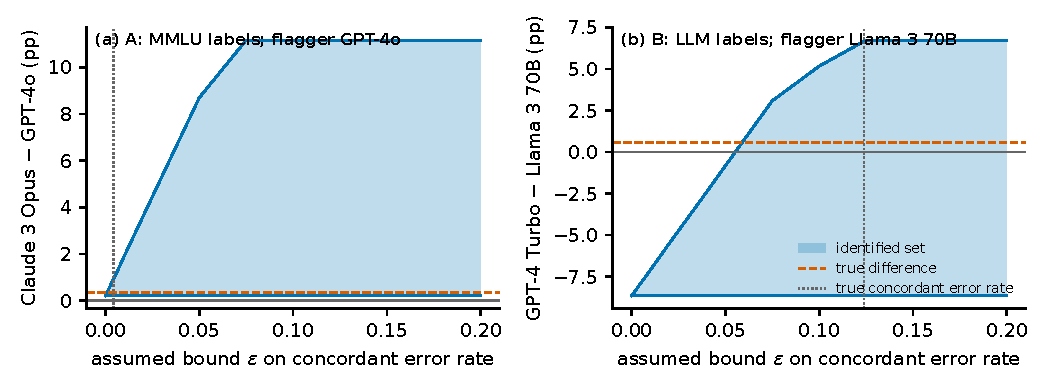
\includegraphics[width=\linewidth]{figures/fig_sensitivity.pdf}
\caption{Sharp identified sets (Theorem~\ref{thm:ident}) for the accuracy difference between a model and the flagger, as a function of the assumed bound $\varepsilon$ on the label-error rate among concordant items. The dashed line marks the true difference and the dotted line the true concordant error rate. The DR value is always the lower endpoint (Corollary~\ref{cor:advantage}).}
\label{fig:sensitivity}
\end{figure}

Figure~\ref{fig:sensitivity} applies Theorem~\ref{thm:ident} to two DR audits as a reader of a published audit would, using only the DR data and an assumed $\varepsilon$.

In Scenario A (flagger GPT-4o), DR reports that Claude~3~Opus is \sensPairDRA~pp more accurate than the flagger; the truth is \sensPairTrueA~pp. Because DR understates advantages over the flagger, the sign of this comparison is identified for every $\varepsilon$.

In Scenario B (flagger Llama~3~70B), DR places GPT-4~Turbo \sensPairDRBabs~pp below the flagger, whereas GPT-4~Turbo is in fact \sensPairTrueB~pp more accurate. For every $\varepsilon$ up to 0.05 the identified set lies entirely below zero, so a reader who trusts a concordant error rate of a few percent would accept the flagger's lead. The set first contains the true difference at $\varepsilon=\sensEpsCoverB$, while the true concordant error rate is \sensTrueRateB. Sensitivity analysis therefore protects a reader only if the assumed $\varepsilon$ is realistic, and DR data cannot tell the reader what is realistic. That is the argument for sampling concordant items. Online Appendix Table~OA.2 reports per-model bounds.

\paragraph{The rate in $m$.} The empirical RMSE of the flagger's estimate (Llama~3~70B, Scenario B) is within a factor of \rateRatioMin--\rateRatioMax{} of the design standard error~\eqref{eq:upper} at every $m$ from 10 to 1{,}000, confirming the $m^{-1/2}$ rate; the lower bound of Theorem~\ref{thm:lower} has the same slope (Online Appendix Figure~OA.1).


%=====================================================================
\section{Related work}
\label{sec:related}
%=====================================================================

\paragraph{Discrepant analysis in diagnostic medicine.} Using a new test to decide which specimens get the reference test, and keeping the old result for the rest, was common practice in the evaluation of nucleic-acid amplification tests in the 1990s.

\emph{The bias.} \citet{hadgu1996discrepancy,hadgu1997bias,hadgu1999discrepant} and \citet{miller1998bias} showed that the procedure biases the new test's sensitivity and specificity upwards. \citet{green1998evaluation} and \citet{lipman1998quantifying} quantified the size of this bias, and \citet{hadgu2000discrepant} reviewed the debate.

\emph{The fixes.} The composite reference standard of \citet{alonzo1999using} and the analysis of \citet{hawkins2001some} restore validity by also sampling concordant results, which is our two-phase design in the clinical setting. Related lines of work cover verification bias \citep{begg1983assessment} and latent-class models for imperfect reference standards \citep{hui1980estimating,walter1988estimation,reitsma2009review}. \citet{limmathurotsakul2012fools} illustrate how an imperfect gold standard can mislead.

\emph{Our contribution relative to this work.} The bias itself is therefore not new. What we add is the analysis that matters for machine learning:
\begin{itemize}
\item an exact identity for any number of models and classes, rather than one binary test;
\item its consequences for rankings and for the flagger, which is itself an evaluated model;
\item lock-in under panels of correlated flaggers;
\item sharp identified sets under the discrepant design;
\item and an optimality theory for the corrective design.
\end{itemize}

\paragraph{Pooling bias in information retrieval.} Test-collection construction in information retrieval faces the same structure. Only documents retrieved by participating systems are judged, and unjudged documents are assumed non-relevant. This favours systems that contributed to the pool and penalises new ones \citep{zobel1998how,buckley2007bias}, which is the retrieval counterpart of our lock-in result. Estimators based on probability sampling of relevance judgments with inverse-probability weights \citep{aslam2006statistical,yilmaz2006estimating} are the retrieval counterpart of our two-phase design. We are not aware of work that carries this experience over to the relabelling of classification and question-answering benchmarks, where the pooled ``systems'' are the evaluated models themselves.

\paragraph{Label errors in test sets.} Confident learning \citep{northcutt2021confident} and model-based annotation-error detection \citep{klie2023annotation,chong2022detecting} made it routine to find label errors with models, and \citet{northcutt2021pervasive} showed that such errors can change benchmark rankings. Several authors note in passing that flag-only review leaves errors unaccounted for. \citet{northcutt2021pervasive} describe their noise-prevalence estimates as ``optimistic in favor of higher capacity models''; \citet{vendrow2025do} call their error counts lower bounds; and \citet{chong2022detecting} warn that cleaning biases benchmarks towards models similar to the cleaner. Section~\ref{sec:practice} documents how widespread the design is. Correlated errors among language models \citep{kim2025correlated} explain why hidden errors are frequent when both the labels and the flagger come from such models. The same correlation is a known problem for aggregating LLM judges \citep{balasubramanian2026dependence} and goes back to the conditional-independence assumption of Dawid--Skene \citep{dawid1979maximum}. \citet{lam2003evaluating} and \citet{chavoshi2026impact} bound the effect of a noisy reference on estimated accuracy. They do not consider an adjudication design in which part of the benchmark is verified, which is what makes our bounds sharp.

\paragraph{Label-efficient and prediction-powered evaluation.} Our estimator is the classical difference estimator \citep{cassel1976some,sarndal1992model}, a form of double sampling \citep{tenenbein1970double,neyman1938contribution}, with the original label as the auxiliary variable. In the language of prediction-powered inference it is PPI \citep{angelopoulos2023prediction,angelopoulos2026ppi} with the original label as the prediction and the flag as a stratifier \citep{fisch2024stratified}, or active inference with flag-dependent inclusion probabilities \citep{zrnic2024active}. \citet{mozer2026ppi} makes the equivalence between PPI and the difference estimator explicit. We claim no novelty for the estimator.

Recent work on evaluating models with few labels uses an autorater's verdict on a model's outputs as the proxy \citep{boyeau2025autoeval,chatzi2024prediction,eyre2025regression,fogliato2024framework,chen2026efficient}. Active testing selects informative test points \citep{sawade2010active,kossen2021active}. In our setting the proxy is the benchmark label that is already there, and the sampling strata are defined by the very disagreement that motivates the audit. The relevant baseline is not a cheaper estimator but a biased design in wide use.


%=====================================================================
\section{Discussion and recommendations}
\label{sec:discussion}
%=====================================================================

\paragraph{Recommendations.} For anyone who relabels a benchmark with model assistance, our results suggest the following.
\begin{enumerate}
\item \emph{Separate the goals.} Adjudicating flagged items cleans a benchmark; accuracy claims need a probability sample that includes concordant items.
\item \emph{Sample concordant items and report the sample}: the flagging rule, $|\Dset|$, the inclusion probabilities, and the concordant items adjudicated with the errors found. The difference estimator of Section~\ref{sec:twophase} is then valid for every model, now or later.
\item \emph{When label errors are rare, report the simultaneous intervals of Theorem~\ref{thm:simultaneous}}, which cover all accuracies, differences and ranking orders; Wald intervals are unreliable there (Section~\ref{sec:emp-sim}).
\item \emph{Do not rank the flagger, or models close to it, on its own audit without correction} (Corollary~\ref{cor:advantage}).
\item \emph{Re-analyse past DR audits with the sensitivity bounds of Theorem~\ref{thm:ident}}, asking how large a concordant error rate would overturn a reported ranking.
\item \emph{Allocate the budget by stratum error rates}: when estimation is the goal, adjudicating every flagged item first is inefficient (Table~\ref{tab:allocation}).
\end{enumerate}

\paragraph{Limitations.} Our reference labels are themselves the output of an annotation process. MMLU-Redux annotators can err, and items with ambiguous or multiple answers were excluded rather than modelled. All results are therefore relative to the adjudication process (Remark~\ref{rem:adjudicator}), as they would be in any real audit.

Scenario A has only \nLabelErrA{} label errors among \nItems{} items, so its estimates of hidden-error counts rest on few events. Scenario B is semi-synthetic: its labels come from a real model's answers to real questions, but no published benchmark was built this way from these models. The HELM predictions come from 5-shot prompting of models released in 2023--2024; stronger or differently prompted models would change the numbers but not the identities.

For other models the rate of the lower bounds depends on how often they repeat the hidden errors. Our simultaneous intervals are valid but certify few adjacent pairs when models are separated by fractions of a point; certifying such rankings needs large concordant samples. Both lower bounds are stated for the flagger's accuracy, with constants that are not tight. The Neyman allocation in Table~\ref{tab:allocation} uses oracle stratum error rates. Our evidence comes from simulated audits of one benchmark and from one published audit. In the published audit (CoNLL-2003) the hidden-error effect on accuracy is small, the reference re-annotation corrected existing labels rather than labelling blind, and the two expert relabelings disagree on many tokens; other benchmarks may show larger or smaller effects. Finally, our literature survey covers 22 studies chosen to span the design space, not a systematic review.

\paragraph{Conclusion.} Using models to decide which benchmark labels to check is efficient for finding errors, and it is here to stay. The accuracies computed afterwards, however, are not estimates of true accuracy. They inflate the flagger by exactly the mass of errors it shares with the benchmark, they can reorder rankings, and they lock in the blind spots of whichever models did the cleaning. A random sample of the items the models agreed on removes all three problems. When hidden errors are common it does so at a rate no design can beat. When they are rare, no design can do much better than DR's own error, but a concordant sample still reveals how large that error might be.


\acks{To be completed by the author, including funding and competing-interest disclosures as required by JMLR.}

\newpage
\appendix
\section{Proofs}
\label{app:proofs}

Throughout, $\Pn$ denotes the proportion of items. Until the proof of Theorem~\ref{thm:lower}, all randomness comes from the phase-two design.

\paragraph{Proof of Proposition~\ref{prop:bias}.} By definition,
\[
\theta^\DR_k-\theta_k=\frac1n\sum_{i=1}^n\big(\1\{M_{ik}=D_i\}-\1\{M_{ik}=Y_i\}\big).
\]
For $i\in\Dset$, $D_i=Y_i$ and the summand is zero. For $i\in\Cset$ with $L_i=Y_i$, $D_i=L_i=Y_i$ and the summand is again zero. For $i\in J$, that is $i\in\Cset$ with $L_i\ne Y_i$, $D_i=L_i$ and the summand is $\1\{M_{ik}=L_i\}-\1\{M_{ik}=Y_i\}$. Summing gives~\eqref{eq:bias}. The naive bias follows from the same computation with $D$ replaced by $L$ on all items: the summand is nonzero only where $L_i\ne Y_i$. Splitting these items into flagged and unflagged ones shows that DR removes exactly the flagged part. \hfill\BlackBox

\paragraph{Proof of Corollary~\ref{cor:flagger}.} For a single flagger, $i\in\Cset$ means $M_{if}=L_i$. On $J$ we also have $L_i\ne Y_i$, so $\1\{M_{if}=L_i\}=1$ and $\1\{M_{if}=Y_i\}=0$. By~\eqref{eq:bias}, $\theta^\DR_f-\theta_f=\Pn(J)$. For any $k$ each summand in~\eqref{eq:bias} lies in $\{-1,0,1\}$ and is nonzero only on $J$, so $|\theta^\DR_k-\theta_k|\le\Pn(J)$. \hfill\BlackBox

\paragraph{Proof of Corollary~\ref{cor:advantage}.} By Proposition~\ref{prop:bias} and Corollary~\ref{cor:flagger},
\[
(\theta^\DR_k-\theta_k)-(\theta^\DR_f-\theta_f)=\Pn(J,M_k=L)-\Pn(J,M_k=Y)-\Pn(J)=-\Pn(J,M_k\ne L)-\Pn(J,M_k=Y),
\]
which is~\eqref{eq:advantage}. Rearranging, $\theta^\DR_k-\theta^\DR_f=(\theta_k-\theta_f)-\Pn(J,M_k\neq L)-\Pn(J,M_k=Y)$. This is negative, so that DR ranks $f$ strictly above $k$, if and only if $\theta_k-\theta_f<\Pn(J,M_k\neq L)+\Pn(J,M_k=Y)$. Adding the requirement $\theta_k>\theta_f$ gives the stated condition. \hfill\BlackBox

\paragraph{Proof of Proposition~\ref{prop:panel}.}
\begin{enumerate}
\item[(a)] $\Dset_G$ is a union over $G$, so it grows with $G$. Hence $\Cset_{G'}\subseteq\Cset_G$, and $J_{G'}=\Cset_{G'}\cap\{L\ne Y\}\subseteq J_G$.
\item[(b)] On $\Cset_G$, every member $g$ satisfies $M_{ig}=L_i$, so the argument of Corollary~\ref{cor:flagger} applies with $J=J_G$. Since all members share the same bias, their pairwise differences are unchanged.
\item[(c)] This is Proposition~\ref{prop:bias} with $\Dset=\Dset_G$. \hfill\BlackBox
\end{enumerate}

\paragraph{Proof of Theorem~\ref{thm:ident}.} Let $y\in\mathcal Y(\eta)$ and $H=\{i\in\Cset:y_i\ne L_i\}$, so that $|H|\le\lfloor\eta n\rfloor$. Since $y=Y$ on $\Dset$ and $y=L$ on $\Cset\setminus H$,
\[
\theta_k(y)-\theta^\DR_k=\frac1n\sum_{i\in H}\big(\1\{M_{ik}=y_i\}-\1\{M_{ik}=L_i\}\big).
\]
Each summand lies in $\{-1,0,1\}$:
\begin{itemize}
\item it equals $-1$ only if $M_{ik}=L_i$;
\item it equals $+1$ only if $M_{ik}=y_i\ne L_i$, which requires $M_{ik}\notin\{L_i,\inv\}$.
\end{itemize}
Hence $\theta_k(y)-\theta^\DR_k\ge-\min\{|H|,|\{i\in\Cset:M_{ik}=L_i\}|\}/n\ge-\min\{\bar\eta,\Pn(\Cset,M_k=L)\}$, and similarly for the upper bound.

\emph{The endpoints are attained.} For the lower endpoint, take $H$ to be $\min\{\lfloor\eta n\rfloor,|\{i\in\Cset:M_{ik}=L_i\}|\}$ items of $\Cset$ with $M_{ik}=L_i$, and set $y_i$ to any label different from $L_i$ (possible since $c\ge2$). For the upper endpoint, take $H$ inside $\{i\in\Cset: M_{ik}\notin\{L_i,\inv\}\}$ and set $y_i=M_{ik}$. Every intermediate multiple of $1/n$ is attained by using fewer items, which proves the equality.

\emph{Pairwise differences.} For a pair $(k,l)$, the difference $\theta_k(y)-\theta_l(y)-(\theta_k^\DR-\theta_l^\DR)$ equals $n^{-1}\sum_{i\in H}g_i(y_i)$, where
\[
g_i(y)=\big(\1\{M_{ik}=y\}-\1\{M_{ik}=L_i\}\big)-\big(\1\{M_{il}=y\}-\1\{M_{il}=L_i\}\big).
\]
Items contribute separately and each uses one unit of the budget $\lfloor\eta n\rfloor$. The maximum is therefore attained by choosing, for each concordant item, the label $y\ne L_i$ that maximises $g_i(y)$, and then keeping the $\lfloor\eta n\rfloor$ items with the largest positive values. The minimum is attained symmetrically. This greedy rule is exact because all weights are equal. \hfill\BlackBox

\paragraph{Proof of Theorem~\ref{thm:unbiased}.} Condition on the phase-one data. The $\pi_i$ are then fixed, and the $R_i$ are independent Bernoulli$(\pi_i)$ variables, independent of the labels. Since $\E[R_i/\pi_i]=1$ and $n^{-1}\sum_i r_{ik}=\theta_k-\theta^L_k$, we get $\E[\hat\theta_k]=\theta^L_k+\theta_k-\theta^L_k=\theta_k$. By independence,
\[
\mathrm{Var}(\hat\theta_k)=n^{-2}\sum_i r_{ik}^2\,\mathrm{Var}(R_i)/\pi_i^2=n^{-2}\sum_i r_{ik}^2(1-\pi_i)/\pi_i ,
\]
and $\E[R_i(1-\pi_i)\pi_i^{-2}r_{ik}^2]=(1-\pi_i)\pi_i^{-1}r_{ik}^2$. The statements for differences follow by linearity. \hfill\BlackBox

\paragraph{Proof of Proposition~\ref{prop:neyman}.} With stratum-constant probabilities, $\sum_k\mathrm{Var}(\hat\theta_k)=n^{-2}\sum_h(1/\pi_h-1)A_h$. This is convex in $(\pi_h)$, and the constraints are linear. The Karush--Kuhn--Tucker conditions give $A_h/\pi_h^2=\lambda' N_h+\mu_h$, where $\mu_h\ge0$ is the multiplier of the constraint $\pi_h\le1$ and is zero when that constraint is slack. Hence $\pi_h=\min\{1,\lambda\sqrt{A_h/N_h}\}$, with $\lambda$ chosen to meet the budget. When neither cap binds, the ratio is $\sqrt{(A_\Cset/N_\Cset)/(A_\Dset/N_\Dset)}=\sqrt{e_\Cset/e_\Dset}$. \hfill\BlackBox

\paragraph{Derivation of~\eqref{eq:upper}.} For the flagger, $r_{if}=-\1\{i\in J\}$ on $\Cset$, and the discordant stratum contributes no variance because $\pi_\Dset=1$. Theorem~\ref{thm:unbiased} gives
\[
\mathrm{Var}(\hat\theta_f)=n^{-2}(1-\pi_\Cset)|J|/\pi_\Cset .
\]
Substituting $\pi_\Cset=m/|\Cset|$ yields $\gamma_n^2\varepsilon_n(1-\pi_\Cset)/m$.

\paragraph{Proof of Theorem~\ref{thm:lower}.} \emph{Two hypotheses.} Fix any law $Q$ of the observables $(X,L,M_1,\dots,M_K)$ with $Q(M_f=L)=\gamma$, and any conditional law of $Y$ on the event $\{M_f\ne L\}$. Let $y^\star(\ell)=(\ell\bmod c)+1\ne\ell$. For $j\in\{0,1\}$, let $P_j$ have observables distributed as $Q$, the fixed conditional law of $Y$ on $\{M_f\neq L\}$, and, on $\{M_f=L\}$,
\[
Y=y^\star(L)\ \text{ with probability } p_j,\qquad Y=L \text{ otherwise},
\]
independently of the observables. Here $p_0=\varepsilon$ and $p_1=\varepsilon-\delta$ with $0<\delta\le\varepsilon/2$. Both laws belong to $\mathcal P(\gamma,\varepsilon)$, and $\theta_f(P_0)-\theta_f(P_1)=-\gamma\delta$, because on $\{M_f=L\}$ the flagger is correct exactly when $Y=L$.

\emph{The two hypotheses are hard to distinguish.} Under both laws, the observables of all items and the reference labels of discordant items have the same distribution. The only difference lies in the revealed labels of adjudicated concordant items. Each such label reveals an independent Bernoulli$(p_j)$ hidden-error indicator, independent of everything observed before the item was selected. By the chain rule for Kullback--Leibler divergence over the sequence of observations (the same argument as Wald's identity for sequential designs), the divergence between the laws of the observed data is
\[
\mathrm{KL}(P_0^{\rm obs}\,\|\,P_1^{\rm obs})=\E_0[N_\Cset]\;\mathrm{kl}(p_0,p_1)\le m\,\mathrm{kl}(p_0,p_1).
\]
Here $N_\Cset$ is the number of concordant adjudications and $\mathrm{kl}$ the Bernoulli divergence. Using $\mathrm{kl}(p_0,p_1)\le(p_0-p_1)^2/\{p_1(1-p_1)\}$, together with $p_1\ge\varepsilon/2$ and $1-p_1\ge1/2$ (since $\varepsilon\le1/2$), we obtain $\mathrm{KL}\le4m\delta^2/\varepsilon$. Choosing $\delta=\sqrt{\varepsilon/(4m)}$, which satisfies $\delta\le\varepsilon/2$ because $m\ge1/\varepsilon$, gives $\mathrm{KL}\le1$.

\emph{Le Cam's two-point argument.} Let $s=\gamma\delta$ and $A=\{|\hat\theta-\theta_0|<s/2\}$. On $A$ we have $|\hat\theta-\theta_1|>s/2$. Hence
\[
\E_0|\hat\theta-\theta_0|+\E_1|\hat\theta-\theta_1|\ge\tfrac s2\big(P_0(A^c)+P_1(A)\big)\ge\tfrac s2\big(1-\mathrm{TV}(P_0^{\rm obs},P_1^{\rm obs})\big).
\]
By the Bretagnolle--Huber inequality, $1-\mathrm{TV}\ge\frac12e^{-\mathrm{KL}}\ge\frac1{2e}$ \citep{tsybakov2009introduction}. Therefore
\[
\max_j\E_j|\hat\theta-\theta_j|\ge\frac{s}{8e}=\frac{\gamma}{16e}\sqrt{\frac{\varepsilon}{m}} .
\]
\emph{The case $m<1/\varepsilon$.} Take $\delta=\varepsilon/2$ instead. Then $\mathrm{KL}\le4m\delta^2/\varepsilon=m\varepsilon<1$, and the same argument gives $\max_j\E_j|\hat\theta-\theta_j|\ge\gamma\varepsilon/(16e)$. Combining the two cases gives the bound $\frac{\gamma}{16e}\min\{\varepsilon,\sqrt{\varepsilon/m}\}$.

\emph{The case $m=0$.} With no concordant adjudication, the same construction with $\delta=\varepsilon$ makes the observed laws identical, so $\E_0|\hat\theta-\theta_0|+\E_1|\hat\theta-\theta_1|=\E_0\big[|\hat\theta-\theta_0|+|\hat\theta-\theta_1|\big]\ge|\theta_0-\theta_1|=\gamma\varepsilon$ by the triangle inequality. The maximum risk is then at least $\gamma\varepsilon/2$: the worst-case error of any estimator based on DR data does not shrink as more discordant items are adjudicated. \hfill\BlackBox

\paragraph{Proof of Theorem~\ref{thm:lowerfp}.} We lower-bound the maximum risk by a Bayes risk. Under hypothesis $j\in\{0,1\}$, let each concordant item be a hidden error independently with probability $p_j$, with $p_0=\varepsilon/2$ and $p_1=\varepsilon/2-\delta$, $0<\delta\le\varepsilon/4$; hidden errors take the label $y^\star(L)$ as in the proof of Theorem~\ref{thm:lower}. Everything observed except the revealed labels of adjudicated concordant items is fixed. Each such label reveals an independent Bernoulli$(p_j)$ indicator, independent of everything observed before the item was selected, and at most $m$ are revealed. As in the proof of Theorem~\ref{thm:lower}, $\mathrm{KL}\le m\,\mathrm{kl}(p_0,p_1)\le m\delta^2/\{p_1(1-p_1)\}\le8m\delta^2/\varepsilon$, using $p_1\ge\varepsilon/4$ and $1-p_1\ge1/2$. Choosing $\delta=\sqrt{\varepsilon/(8m)}$, which satisfies $\delta\le\varepsilon/4$ because $m\ge2/\varepsilon$, gives $\mathrm{KL}\le1$.

Write $\theta_f(J)=c-|J|/n$, where $c$ is fixed. Let $m_s\le m$ be the number of adjudicated concordant items and $h$ the number of hidden errors among them, and write $|J|=h+W$, with $W$ the number of hidden errors among the $N_\Cset-m_s$ unadjudicated concordant items. Conditionally on the observed data, the indicators of the unadjudicated items are still independent Bernoulli$(p_j)$, so $\E_j[W\mid\text{data}]=(N_\Cset-m_s)p_j$. By Jensen's inequality, for any estimator $\hat\theta$,
\[
\E_j\big[|\hat\theta-\theta_f(J)|\,\big|\,\text{data}\big]\ge|\hat\theta-\mu_j|,\qquad\mu_j=c-\{h+(N_\Cset-m_s)p_j\}/n .
\]
The centres $\mu_0,\mu_1$ depend on the data, but $|\mu_0-\mu_1|=(N_\Cset-m_s)\delta/n\ge s:=(N_\Cset-m)\delta/n$ pointwise. The two-point argument of Theorem~\ref{thm:lower}, with $A=\{|\hat\theta-\mu_0|<s/2\}$, therefore gives a Bayes risk of at least $\frac12\sum_j\E_j|\hat\theta-\theta_f(J)|\ge s/(8e)$.

Finally, $|J|$ is Binomial$(N_\Cset,p_j)$ with mean at most $\varepsilon N_\Cset/2$. By the multiplicative Chernoff bound, $P(|J|>\varepsilon N_\Cset)\le e^{-\varepsilon N_\Cset/6}$. Taking $\hat\theta\in[0,1]$ without loss of generality, so that the loss is at most one, the maximum risk over $\mathcal J(\varepsilon)$ is at least the Bayes risk minus $e^{-\varepsilon N_\Cset/6}$. Substituting $s/(8e)=\frac{N_\Cset-m}{n}\sqrt{\varepsilon/(8m)}/(8e)$ gives the claim. \hfill\BlackBox

\paragraph{Proof of Theorem~\ref{thm:simultaneous}.} Under Poisson sampling, conditionally on $m$, the sampled concordant items form a simple random sample of size $m$ from $\Cset$, so $h$ follows the hypergeometric distribution with parameters $(|\Cset|,K,m)$. The function $k\mapsto\mathrm{HG}(h;|\Cset|,k,m)$ is non-increasing, so $\{K>U\}=\{\mathrm{HG}(h;|\Cset|,K,m)\le\alpha\}$. Since $\mathrm{HG}(\cdot;|\Cset|,K,m)$ is the distribution function of $h$, we have $P(\mathrm{HG}(h;|\Cset|,K,m)\le\alpha)\le\alpha$, hence $P(K\le U)\ge1-\alpha$. On the event $K\le U$, the unsampled concordant items contain $K-h\le U-h=B$ label errors. The true label vector agrees with $Y$ on $A$ by definition, so it lies in $\mathcal Y_B$. Every $I_k$ and $I_{kl}$ is a range of a function over $\mathcal Y_B$, and therefore contains the corresponding true value on that event; this gives simultaneous coverage. The greedy computation is that of Theorem~\ref{thm:ident}: items in $\Cset\setminus S$ contribute separately, each uses one unit of the budget $B$, and labels on $A$ are fixed. \hfill\BlackBox

\paragraph{Proof of Proposition~\ref{prop:width}.} By the proof of Theorem~\ref{thm:ident}, each changed label moves $\theta_k$ by at most $1/n$ and $\theta_k-\theta_l$ by at most $2/n$, in either direction, which gives the width bounds. If $h=0$, then $\mathrm{HG}(0;N,k,m)=\binom{N-k}{m}/\binom{N}{m}\le(1-k/N)^m\le e^{-km/N}$, which is at most $\alpha$ once $k\ge N\log(1/\alpha)/m$. Hence $U\le|\Cset|\log(1/\alpha)/m$. Since the sampled items carry no label errors, $\mathcal Y_B$ is contained in the set $\mathcal Y(\eta)$ of Theorem~\ref{thm:ident} with $\eta=U/n\le\gamma_n\log(1/\alpha)/m$, so the intervals are contained in its bounds. \hfill\BlackBox

\paragraph{Proof of Lemma~\ref{lem:width}.} Let $H_0$ be the configuration $J=\emptyset$ and $H_1$ a uniformly random hidden-error set of size $k^\star$ in $\Cset$ (on $\Cset$ the flagger agrees with $L$, so every hidden error lowers $\theta_f$ by exactly $1/n$). Then $\theta_f(H_1)=\theta_f(H_0)-k^\star/n$, a deterministic difference. Let $Z$ denote the observed data. Under $H_0$ the sample never contains an error. Under $H_1$ the sample contains no error with probability $q=\binom{N-k^\star}{m}/\binom Nm\ge2\alpha$. Conditionally on that event, the sampled set is uniform over $m$-subsets (each subset avoids a uniformly random $k^\star$-set with the same probability), and the revealed labels all equal $L$; hence $Z$ has the same conditional law as under $H_0$, which we call $Q$.

Coverage at least $1-\alpha$ for every configuration implies coverage at least $1-\alpha$ averaged over the random configuration of $H_1$. So $P_1(\theta_f(H_1)\in I(Z),\ \text{no error})\ge q-\alpha$, and therefore $Q(\theta_f(H_1)\in I)\ge(q-\alpha)/q\ge\frac12$. Also $Q(\theta_f(H_0)\in I)\ge1-\alpha$. Hence $Q$ puts probability at least $\frac12-\alpha$ on intervals containing both values, and $\E_Q|I|\ge(\frac12-\alpha)k^\star/n$.

For the bound on $k^\star$: $\binom{N-k}{m}/\binom Nm=\prod_{i=0}^{m-1}(N-k-i)/(N-i)\ge(1-k/(N-m+1))^m$. This is at least $2\alpha$ whenever $k\le(N-m+1)(1-(2\alpha)^{1/m})$. Since $1-e^{-x}\ge x/(1+x)$, the latter is at least $(N-m+1)x/(1+x)$. \hfill\BlackBox

\paragraph{Proof of Proposition~\ref{prop:rule}.} On $\Cset$, $r_{ik}=\1\{M_{ik}=Y_i\}-\1\{M_{ik}=L_i\}$ is $-1$ on $J\cap\{M_k=L\}$, $+1$ on $J\cap\{M_k=Y\}$ and $0$ elsewhere. Proposition~\ref{prop:bias} gives the DR bias $\gamma_n(a_k-c_k)$. Theorem~\ref{thm:unbiased} with $\pi_\Dset=1$ gives the variance $n^{-2}(1-\pi_\Cset)\pi_\Cset^{-1}|\Cset|(a_k+c_k)=\gamma_n^2(1-\pi_\Cset)(a_k+c_k)/m$. Comparing the squared bias with this variance gives the threshold. \hfill\BlackBox

\section{Additional results}

Table~\ref{tab:conllentity} gives the CoNLL-2003 re-analysis on entity tokens. The full Scenario A flagger results and per-model sensitivity bounds are in the Online Appendix (Tables~OA.1 and OA.2).

\begin{table}[H]
\centering
\scriptsize
\begin{tabular}{lrrrrrrr}
\toprule
 & \multicolumn{2}{c}{Accuracy (\%)} & \multicolumn{3}{c}{DR bias (pp)} & \multicolumn{2}{c}{Rank} \\
\cmidrule(lr){2-3}\cmidrule(lr){4-6}\cmidrule(lr){7-8}
Model & CoNLL++ & DR & total & hidden & disagr. & true & DR \\
\midrule
RoBERTa-large (J.-B.) & 95.87 & 93.35 & -2.52 & -0.10 & -2.42 & 1 & 1 \\
BERT-large (dbmdz) & 94.94 & 93.00 & -1.95 & +0.26 & -2.20 & 2 & 2 \\
BERT-large (dslim) & 94.58 & 92.58 & -2.00 & +0.10 & -2.09 & 3 & 3 \\
BERT-base (dslim) & 94.22 & 92.48 & -1.74 & +0.26 & -2.00 & 4 & 4 \\
DistilBERT (elastic) & 93.08 & 91.33 & -1.75 & +0.34 & -2.09 & 5 & 5 \\
Florian (2003) & 90.97 & 88.60 & -2.36 & +0.11 & -2.47 & 6 & 6 \\
Chieu (2003) & 89.22 & 87.82 & -1.40 & +0.61 & -2.01 & 7 & 7 \\
Klein (2003) & 88.04 & 86.94 & -1.10 & +0.78 & -1.89 & 8 & 8 \\
Zhang (2003) & 87.65 & 85.95 & -1.70 & +0.23 & -1.93 & 9 & 9 \\
Carreras (a) (2003) & 87.02 & 85.46 & -1.57 & +0.23 & -1.80 & 10 & 10 \\
Curran (2003) & 86.86 & 85.26 & -1.60 & +0.31 & -1.91 & 11 & 11 \\
Munro (2003) & 86.61 & 85.08 & -1.53 & +0.36 & -1.89 & 12 & 12 \\
Mayfield (2003) & 86.47 & 84.86 & -1.62 & +0.53 & -2.14 & 13 & 13 \\
Bender (2003) & 85.41 & 83.80 & -1.60 & +0.10 & -1.70 & 14 & 14 \\
McCallum (2003) & 84.99 & 83.63 & -1.36 & +0.58 & -1.93 & 15 & 15 \\
Carreras (b) (2003) & 84.15 & 82.52 & -1.63 & +0.32 & -1.95 & 16 & 16 \\
Hendrickx (2003) & 83.49 & 81.70 & -1.79 & +0.16 & -1.95 & 17 & 18 \\
Wu (2003) & 83.43 & 81.75 & -1.68 & +0.50 & -2.18 & 18 & 17 \\
De Meulder (2003) & 81.34 & 79.35 & -2.00 & +0.16 & -2.15 & 19 & 19 \\
Whitelaw (2003) & 81.11 & 79.29 & -1.82 & +0.28 & -2.11 & 20 & 20 \\
Hammerton (2003) & 56.87 & 55.61 & -1.26 & +0.51 & -1.78 & 21 & 21 \\
\bottomrule
\end{tabular}

\caption{CoNLL-2003 re-analysis restricted to the \cnEnt{} tokens whose original or reference label is an entity (Section~\ref{sec:emp-conll}). Columns as in Table~\ref{tab:conll}.}
\label{tab:conllentity}
\end{table}

\FloatBarrier

\vskip 0.2in
\bibliography{refs}

\end{document}
